
\documentclass[conference]{IEEEtran}
\usepackage[utf8]{inputenc}
\usepackage[T1]{fontenc}
\usepackage[spanish,es-tabla,es-noshorthands]{babel}
\usepackage{array}
\usepackage{amsmath,amssymb}
\usepackage{url}
\usepackage{graphicx}
\usepackage{float}
\usepackage{cite}
\usepackage{tikz}
\usetikzlibrary{shapes.multipart,shapes.geometric,arrows.meta,calc,positioning,fit}
\usepackage[colorlinks=true,linkcolor=blue!60!black,citecolor=blue!60!black,urlcolor=blue!60!black]{hyperref}
\hbadness=10000 \vbadness=10000 \hfuzz=3pt
\hyphenation{si-mu-la-ción pro-ce-sa-dor}

\tikzset{
  ttl/.style={text width=5.2cm, align=center, font=\fontsize{5.5}{6.2}\selectfont\sffamily\bfseries},
  act/.style={draw, rounded corners=2pt, text width=2.4cm, align=center, font=\fontsize{5}{5.6}\selectfont\sffamily, inner sep=2pt, fill=blue!6},
  alt/.style={draw, rounded corners=2pt, text width=1.9cm, align=center, font=\fontsize{5}{5.6}\selectfont\sffamily, inner sep=2pt, fill=red!6},
  gd/.style={text width=1.55cm, align=right, font=\fontsize{4.6}{5.2}\selectfont\sffamily\itshape, inner sep=1pt},
  dec/.style={diamond, draw, inner sep=0pt, minimum width=0.5cm, minimum height=0.32cm, fill=yellow!15},
  ini/.style={circle, fill=black, inner sep=0pt, minimum size=5pt},
  fin/.style={circle, draw, fill=black, inner sep=0pt, minimum size=5pt, line width=0.8pt, double=white, double distance=0.5pt},
  lbl/.style={font=\fontsize{4.6}{5}\selectfont\sffamily, inner sep=1pt},
  cls/.style={rectangle split, rectangle split parts=3, draw, text width=3.0cm, align=left, inner sep=1.6pt,
    font=\fontsize{5.5}{6.2}\selectfont\sffamily, fill=white},
  comp/.style={thin, {Diamond[length=4pt,width=3pt]}-},
  agg/.style={thin, {Diamond[open,length=4pt,width=3pt]}-},
  asoc/.style={thin},
  herencia/.style={thin, -{Triangle[open,length=5pt,width=4pt]}},
  dep/.style={thin, dashed, ->, >=Stealth}
}
\begin{document}
\title{Avance 1: Propuesta y Modelado de un Minikernel con Arquitectura de Microkernel\\
\large Dise\~no y simulaci\'on web \textemdash{} Sistemas Operativos}
\author{
\begin{tabular}[t]{c@{\hspace{2.5em}}c}
\textbf{Gabriela Mart\'inez Silva} & \textbf{Kaleth Molina D\'iaz}\\
C\'odigo 20231020205 & C\'odigo 20232020096\\[4pt]
\textbf{Carol Stefanya Velasco Rodr\'iguez} & \textbf{Camilo Andr\'es Gamez Camino}\\
C\'odigo 20231020215 & C\'odigo 20231020193
\end{tabular}\\[6pt]
Universidad Distrital Francisco Jos\'e de Caldas\\
Sistemas Operativos, Grupo 82\\
Docente: Gerald Breek Fuenmayor Rivadeneira\\
Bogot\'a, noviembre de 2026
}
\maketitle

\begin{abstract}
Este documento presenta el primer avance del proyecto de diseño y simulación web de un minikernel con arquitectura de microkernel. Se define una arquitectura en la que el núcleo solo ofrece planificación básica, comunicación entre procesos (IPC) e interrupciones, y cinco servidores en espacio de usuario (procesos, memoria, archivos, E/S y seguridad) se comunican únicamente mediante mensajes. Se documentan 26 requerimientos funcionales y 10 no funcionales, 14 casos de uso con su diagrama de casos de uso, un diagrama de clases con 22 clases y un análisis de trazabilidad entre requerimientos y casos de uso. Las tablas y diagramas se generan desde una misma fuente de datos y se verifican de forma automática para evitar inconsistencias.
\end{abstract}
\renewcommand{\IEEEkeywordsname}{Palabras clave}
\begin{IEEEkeywords}
microkernel, simulación web, Spring Boot, UML, requerimientos, casos de uso, trazabilidad
\end{IEEEkeywords}

\section{Introducción}
Los sistemas operativos deben equilibrar rendimiento, seguridad y facilidad de mantenimiento. Frente a los núcleos monolíticos, la arquitectura de microkernel conserva dentro del núcleo solo lo indispensable (planificación básica, comunicación entre procesos e interrupciones) y traslada el resto de los servicios a procesos que se ejecutan en espacio de usuario y se comunican por mensajes~\cite{tanenbaum,silberschatz}. Esta separación mejora el aislamiento de fallos y la extensibilidad del sistema, a cambio de una mayor sobrecarga de comunicación.

Comprender cómo cooperan la planificación de procesos, la administración de memoria, el sistema de archivos, la entrada/salida y la seguridad resulta difícil si solo se estudia de forma teórica. Un simulador interactivo permite observar estos mecanismos paso a paso, modificar sus parámetros y comparar políticas en condiciones controladas.

Este trabajo presenta el diseño de un simulador web de un minikernel basado en microkernel. El documento corresponde al primer avance del proyecto (propuesta y modelado) y sus aportes son: (i) una arquitectura en capas con un contrato de mensajes entre servidores, (ii) la especificación de requerimientos funcionales y no funcionales, (iii) un conjunto de casos de uso con su diagrama UML, (iv) un diagrama de clases y (v) un análisis de trazabilidad que relaciona requerimientos, casos de uso y clases. Los requerimientos se redactan en términos de entrada, procesamiento, salida y restricciones, siguiendo la práctica de ISO/IEC/IEEE 29148~\cite{iso29148}, y el modelado emplea UML~\cite{uml}.

El resto del documento se organiza así: la Sección~\ref{sec:alcance} fija el alcance y los supuestos; la Sección~\ref{sec:arq} describe la arquitectura; la Sección~\ref{sec:req} resume los requerimientos; la Sección~\ref{sec:cu} presenta los casos de uso; la Sección~\ref{sec:clases} el modelo de clases; la Sección~\ref{sec:traza} el análisis de trazabilidad; y la Sección~\ref{sec:plan} los siguientes pasos. Todas las tablas se incluyen en los anexos.

\section{Alcance y supuestos}\label{sec:alcance}
El simulador cubre cinco módulos: procesos, memoria, archivos, entrada/salida y seguridad. Se adoptan las siguientes decisiones de diseño, que el equipo podrá ajustar en los avances siguientes:
\begin{itemize}
\item \textbf{Plataforma.} Backend en Java 17 con Spring Boot 3, que ejecuta el simulador (Kernel y servidores) y lo expone por WebSocket (STOMP) y REST. El cliente web, construido con Thymeleaf y JavaScript, solo dibuja el estado y envía comandos.
\item \textbf{Persistencia.} Base de datos relacional con Spring Data JPA (H2 en desarrollo y PostgreSQL opcional) para usuarios, bitácoras, parámetros de disco y sistema de archivos (RF-26).
\item \textbf{Ejecución de los servidores.} Cada servidor es un componente con su propio hilo y una cola \texttt{BlockingQueue<IPCMessage>}; solo el Kernel conoce todas las colas y ningún servidor se inyecta en otro.
\item \textbf{Programas simulados.} Cada aplicación es una lista de ráfagas e instrucciones propias del simulador (cómputo, E/S, \texttt{SEND}, \texttt{RECV}, \texttt{WAIT}, \texttt{SIGNAL}); no se ejecuta código arbitrario.
\item \textbf{Tiempo.} La simulación avanza por ticks de reloj; todas las métricas se expresan en ticks.
\item \textbf{Documentación pendiente.} El mapa de navegación web y el modelo de persistencia detallado se entregarán con los avances siguientes (Sección~\ref{sec:plan}).
\end{itemize}
Se eligió Java porque las clases del modelo UML se traducen casi directamente a clases del sistema y porque una base de datos relacional responde de forma natural a los requerimientos de persistencia.

\section{Arquitectura propuesta}\label{sec:arq}
La arquitectura es un microkernel con cinco capas (Fig.~\ref{fig:arq}, anexo~\ref{ax:arq}). El \texttt{Kernel} conserva únicamente tres servicios: planificación básica de la CPU (\texttt{Scheduler}), enrutamiento de mensajes IPC (\texttt{IPCMessage}) y despacho de interrupciones (\texttt{InterruptController}). Los demás servicios viven en servidores de espacio de usuario que heredan de la clase abstracta \texttt{Server} y solo reciben y envían mensajes. Así, un fallo en un servidor no corrompe el núcleo, como corresponde a un diseño de microkernel (RF-24, RNF-01).

La Fig.~\ref{fig:arq} (anexo~\ref{ax:arq}) muestra las capas. La interfaz web no invoca a los servidores directamente: la API de Spring Boot convierte cada comando del usuario en un \texttt{IPCMessage} que entrega al \texttt{Kernel}. El anexo~\ref{ax:msg} (Tabla~\ref{tab:msg}) define el contrato de mensajes; cada tipo tiene un único servidor receptor.

\section{Requerimientos}\label{sec:req}
Se definen 26 requerimientos funcionales (RF) agrupados por módulo: Procesos (9), Memoria (4), Archivos (3), E/S (4), Seguridad (3), Núcleo (3). Cada uno se describe con su entrada, procesamiento, salida, restricciones y los casos de uso que lo ejercitan (anexo~\ref{ax:rf}, Tablas~\ref{tab:rf-procesos} a~\ref{tab:rf-nucleo}).

Los 10 requerimientos no funcionales (RNF) fijan atributos de calidad: arquitectura microkernel, plataforma, rendimiento, reproducibilidad, usabilidad, persistencia, seguridad de la simulación, mantenibilidad, coherencia entre documentos y código, y aislamiento por sesión. Cada uno incluye cómo se verificará (anexo~\ref{ax:rnf}, Tabla~\ref{tab:rnf}).

\section{Casos de uso}\label{sec:cu}
Se especifican 14 casos de uso que cubren los cinco módulos: Procesos (4), Memoria (2), Archivos (2), E/S (3) y Seguridad (3). La Fig.~\ref{fig:cu} (anexo~\ref{ax:cud}) muestra el diagrama de casos de uso, con los actores que interactúan con el simulador:
\begin{itemize}
\item \textbf{Usuario:} opera la simulación y configura sus parámetros.
\item \textbf{Usuario Root:} especialización del usuario con permisos de administración (formatear el sistema de archivos y consultar la auditoría).
\item \textbf{Proceso simulado:} solicita memoria, E/S, comunicación y sincronización.
\item \textbf{Kernel:} genera los ticks que activan la planificación.
\item \textbf{Servidor:} cualquier servidor que consulta permisos al \texttt{SecurityServer}.
\end{itemize}
Las relaciones \guillemotleft include\guillemotright{} reflejan comportamiento compartido: crear un proceso incluye asignar memoria (CU-01 a CU-05), y las operaciones que exigen autorización incluyen la verificación de permisos (CU-13). Cada especificación del anexo~\ref{ax:cu} indica actor, precondiciones, flujo principal, flujos alternos, postcondición y las clases y métodos que participan.

\section{Diagramas de actividad}\label{sec:act}
Para cada caso de uso se elaboró un diagrama de actividad UML (Figs.~\ref{fig:act-cu01} a~\ref{fig:act-cu14}, anexo~\ref{ax:act}). Cada diagrama parte del nodo inicial (círculo negro), muestra las acciones del flujo principal (rectángulos redondeados), las decisiones con su condición de guarda (rombos con salidas «sí» y «no»), las acciones del flujo alterno y los nodos finales. Los diagramas se generan a partir del flujo principal y los flujos alternos de las Tablas~\ref{tab:cu1} y~\ref{tab:cu2}, por lo que no pueden contradecirlos.


\section{Diagrama de clases}\label{sec:clases}
La Fig.~\ref{fig:clases} (anexo~\ref{ax:cls}) muestra el modelo de clases con 22 clases. Incluye las clases centrales del núcleo y de los servidores (\texttt{Kernel}, \texttt{PCB}, \texttt{MemoryManager}, \texttt{FileManager}, \texttt{DeviceDriver}, \texttt{SecurityController} e \texttt{IPCMessage}) y las clases de apoyo necesarias para los casos de uso.

Las relaciones principales son las siguientes. El \texttt{Kernel} compone un \texttt{Scheduler} y un \texttt{InterruptController} y agrega los servidores. Los cinco servidores heredan de \texttt{Server}, que intercambia \texttt{IPCMessage}. Cada servidor posee un gestor de dominio (\texttt{ProcessServer} con \texttt{PCB}, \texttt{MemoryServer} con \texttt{MemoryManager}, \texttt{FileServer} con \texttt{FileManager}, \texttt{IOServer} con \texttt{DeviceDriver} y \texttt{SecurityServer} con \texttt{SecurityController}). El \texttt{MemoryManager} compone particiones, el \texttt{FileManager} el árbol de \texttt{FileNode} y el \texttt{SecurityController} los usuarios y los eventos de auditoría. El \texttt{ProcessServer} usa el \texttt{BankerAlgorithm} y los \texttt{Semaphore}, y el \texttt{IOServer} programa al \texttt{DMAController}. Las flechas discontinuas son dependencias de uso.

\section{Trazabilidad entre requerimientos y casos de uso}\label{sec:traza}
Para evitar inconsistencias entre requerimientos, casos de uso y clases, las tablas, las matrices y los diagramas se generan con un único programa a partir de una sola fuente de datos, y este valida las reglas del anexo~\ref{ax:traza} (Tabla~\ref{tab:verif}). Se mantiene una matriz de requerimientos funcionales contra casos de uso (Tabla~\ref{tab:traza}) con el nombre completo de cada elemento. Del análisis se concluye lo siguiente.

\textbf{Cobertura.} Los 26 requerimientos funcionales se enlazan con al menos un caso de uso y los 14 casos de uso responden a al menos un requerimiento, de modo que no hay requerimientos hu\'erfanos ni casos de uso sin justificaci\'on (Tabla~\ref{tab:traza}). En total existen 41 v\'inculos RF--CU, es decir, 1.6 casos de uso por requerimiento en promedio; la Tabla~\ref{tab:cob} resume la cobertura por m\'odulo.

\textbf{Concentraci\'on.} 4 requerimientos se ejercitan en tres o m\'as casos de uso (RF-22, RF-23, RF-24, RF-26). Son los transversales de seguridad y de n\'ucleo, por lo que un cambio en ellos tiene el mayor impacto: por ejemplo, modificar RF-22 obligar\'ia a revisar CU-01, CU-07, CU-08, CU-13.

\textbf{Casos de uso m\'as cargados.} CU-02 cubre 7 requerimientos, el m\'aximo; conviene priorizarlo en las pruebas de integraci\'on.

\textbf{Riesgo por cobertura \'unica.} 18 requerimientos (RF-01, RF-02, RF-03, RF-04, RF-06, RF-07, RF-08, RF-09, RF-10, RF-12, RF-14, RF-15, RF-16, RF-17, RF-18, RF-19, RF-20, RF-21) dependen de un solo caso de uso para su validaci\'on. Si ese caso falla o cambia, no queda otra evidencia, por lo que en los avances siguientes se agregar\'an pruebas dedicadas a cada uno.

Las clases \texttt{AuditEvent, FileNode, IPCMessage, Server, User} no aparecen como operaciones en los casos de uso porque son la clase base abstracta o estructuras de datos sin comportamiento propio; se usan a través de las demás clases.

\section{Plan de los siguientes avances}\label{sec:plan}
\begin{itemize}
\item \textbf{Documentación final pendiente:} mapa de navegación web, modelo de persistencia (tablas relacionales para usuarios, logs, discos y sistema de archivos) y revisión cruzada final.
\item \textbf{Avance 2:} prototipo web de los módulos de Procesos y Memoria, que implementa los RF-01 a RF-13 sobre el Kernel y la mensajería del anexo~\ref{ax:msg}.
\item \textbf{Entrega final:} módulos de Archivos, E/S y Seguridad, persistencia, pruebas de integración y sustentación.
\end{itemize}

\section{Conclusiones}
El primer avance deja definidos la arquitectura de microkernel, el contrato de mensajes y el modelo de clases del simulador, con trazabilidad completa entre 26 requerimientos funcionales, 14 casos de uso y 22 clases. El análisis identificó los requerimientos transversales de seguridad y núcleo como los de mayor impacto y los requerimientos con un único caso de uso como los que requieren pruebas adicionales. Generar la documentación desde una fuente única reduce el riesgo de inconsistencias y facilita mantenerla alineada con el código.

\clearpage
\renewcommand{\appendixname}{Anexo}
\appendices
\section{Arquitectura propuesta}\label{ax:arq}
La Fig.~\ref{fig:arq} presenta la arquitectura en capas descrita en la Sección~\ref{sec:arq}.

\begin{figure*}[!t]
\centering
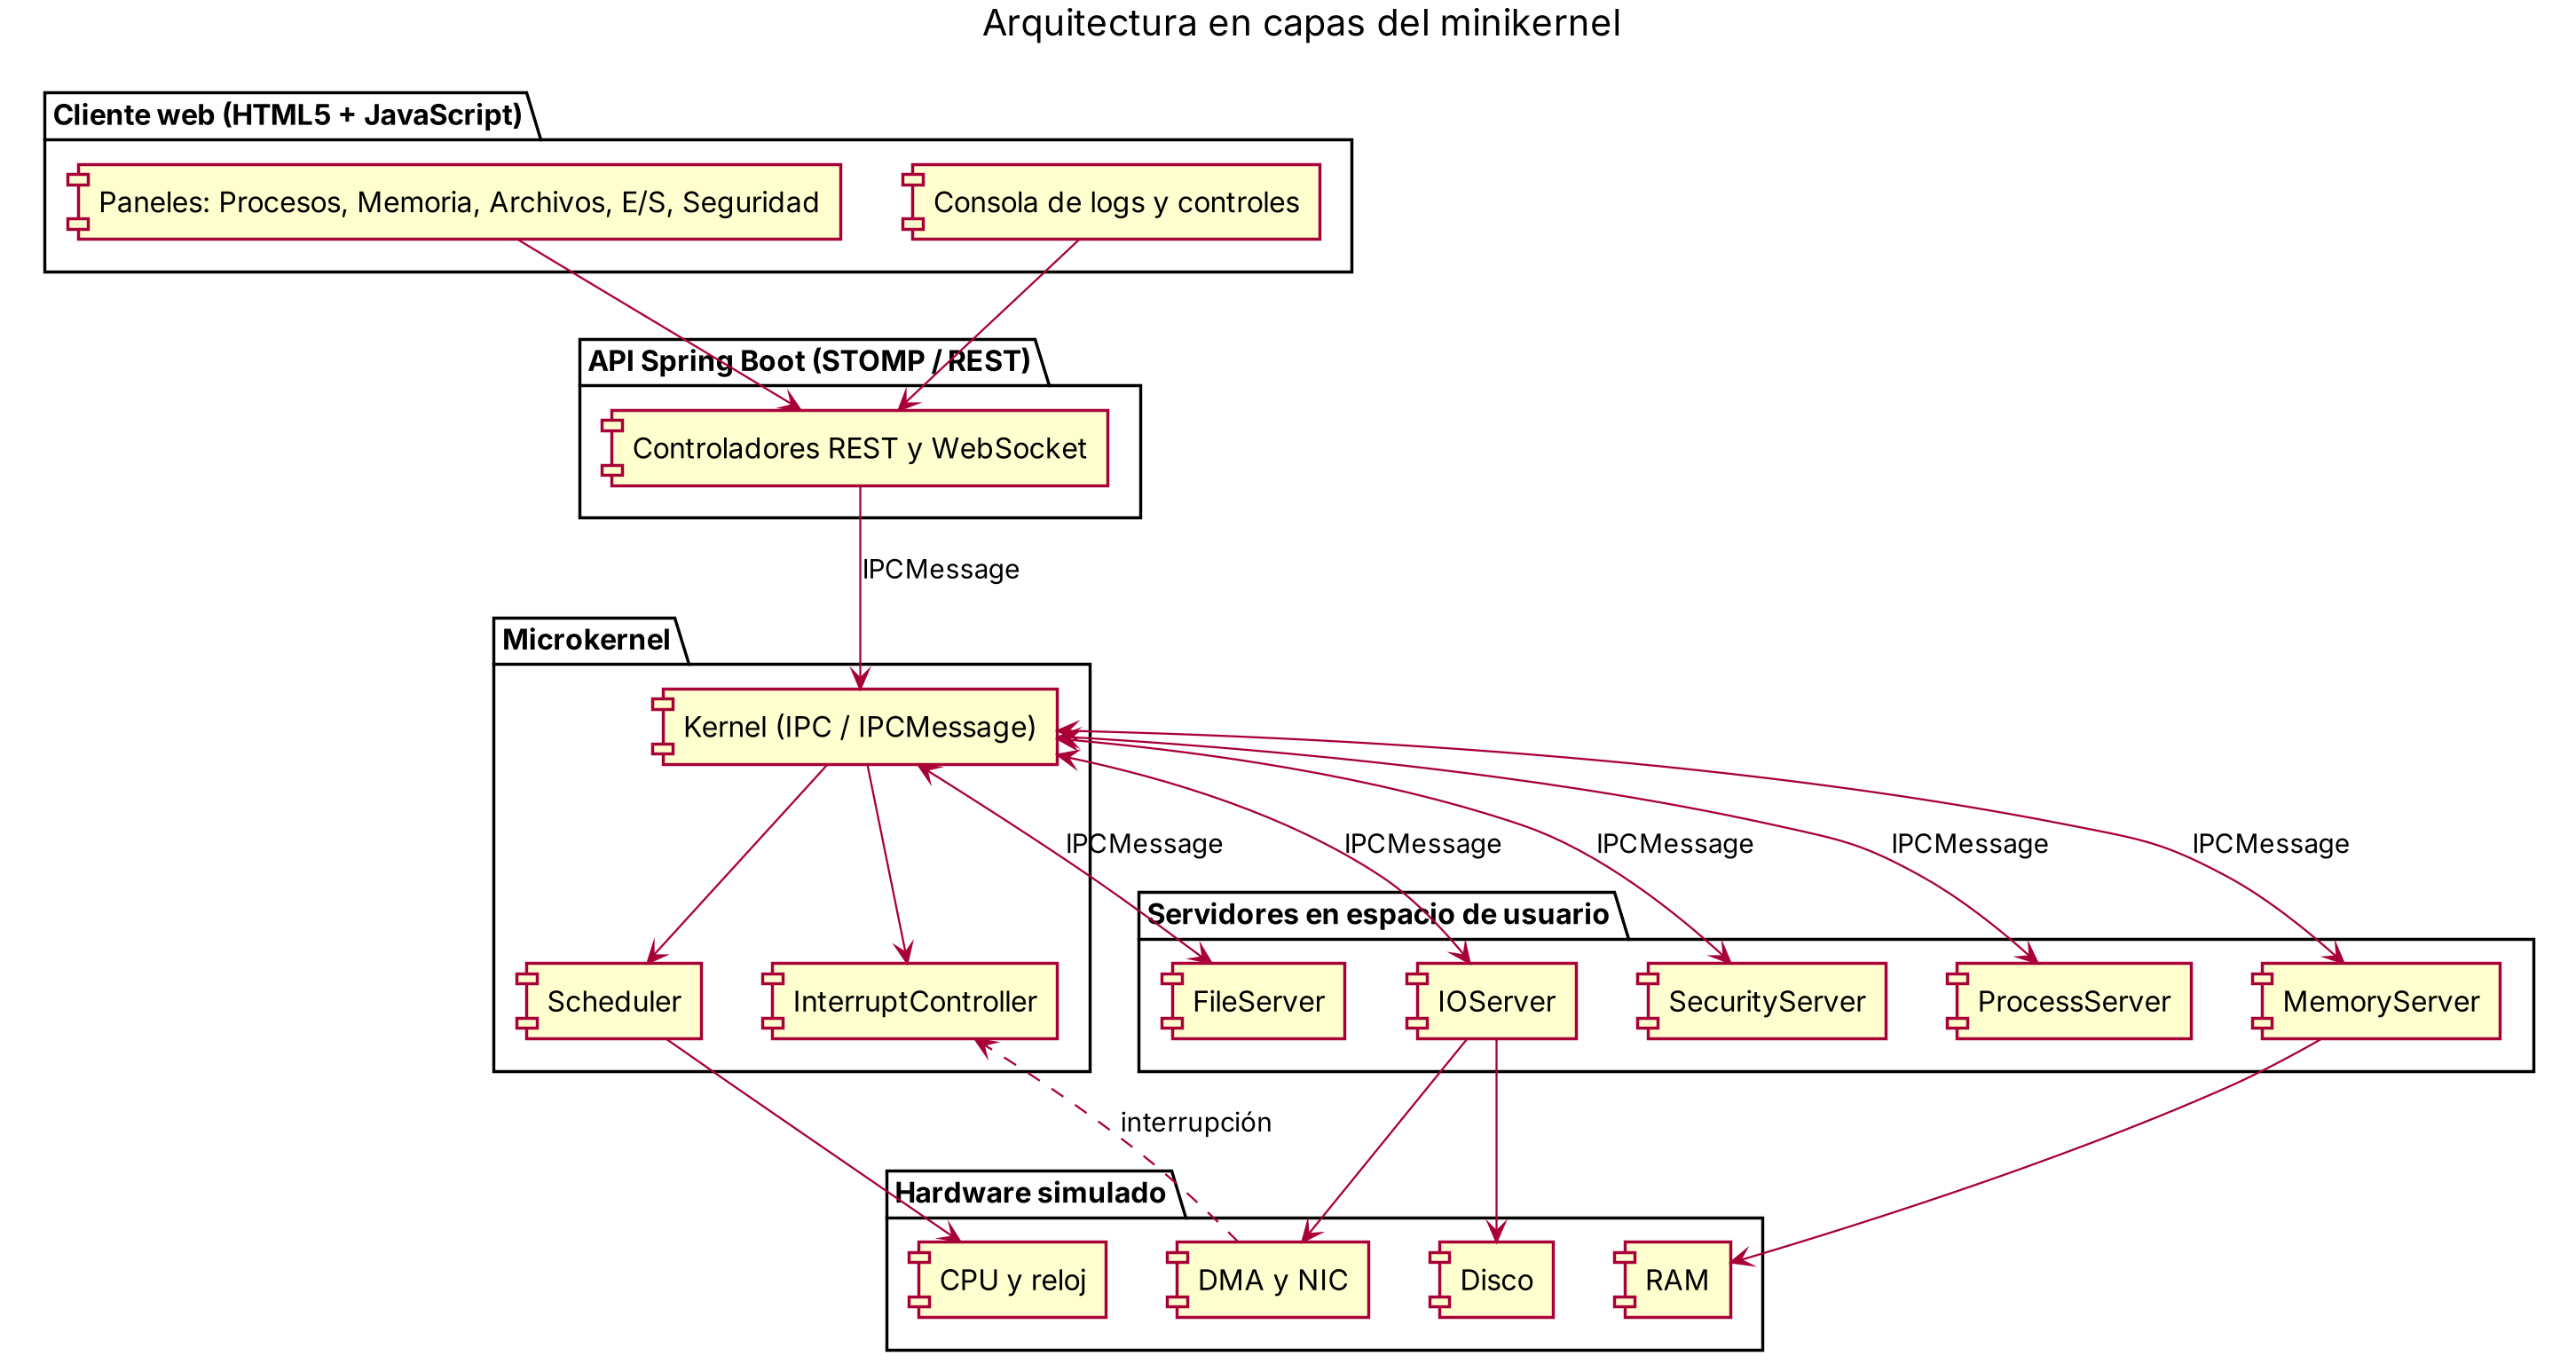
\includegraphics[width=0.95\textwidth,keepaspectratio]{figuras/arquitectura.png}
\caption{Arquitectura en capas propuesta. Los servidores solo se comunican mediante el Kernel.}
\label{fig:arq}
\end{figure*}

\section{Diagrama de casos de uso}\label{ax:cud}
La Fig.~\ref{fig:cu} muestra los actores y los casos de uso descritos en la Sección~\ref{sec:cu}.

\begin{figure*}[!p]
\centering
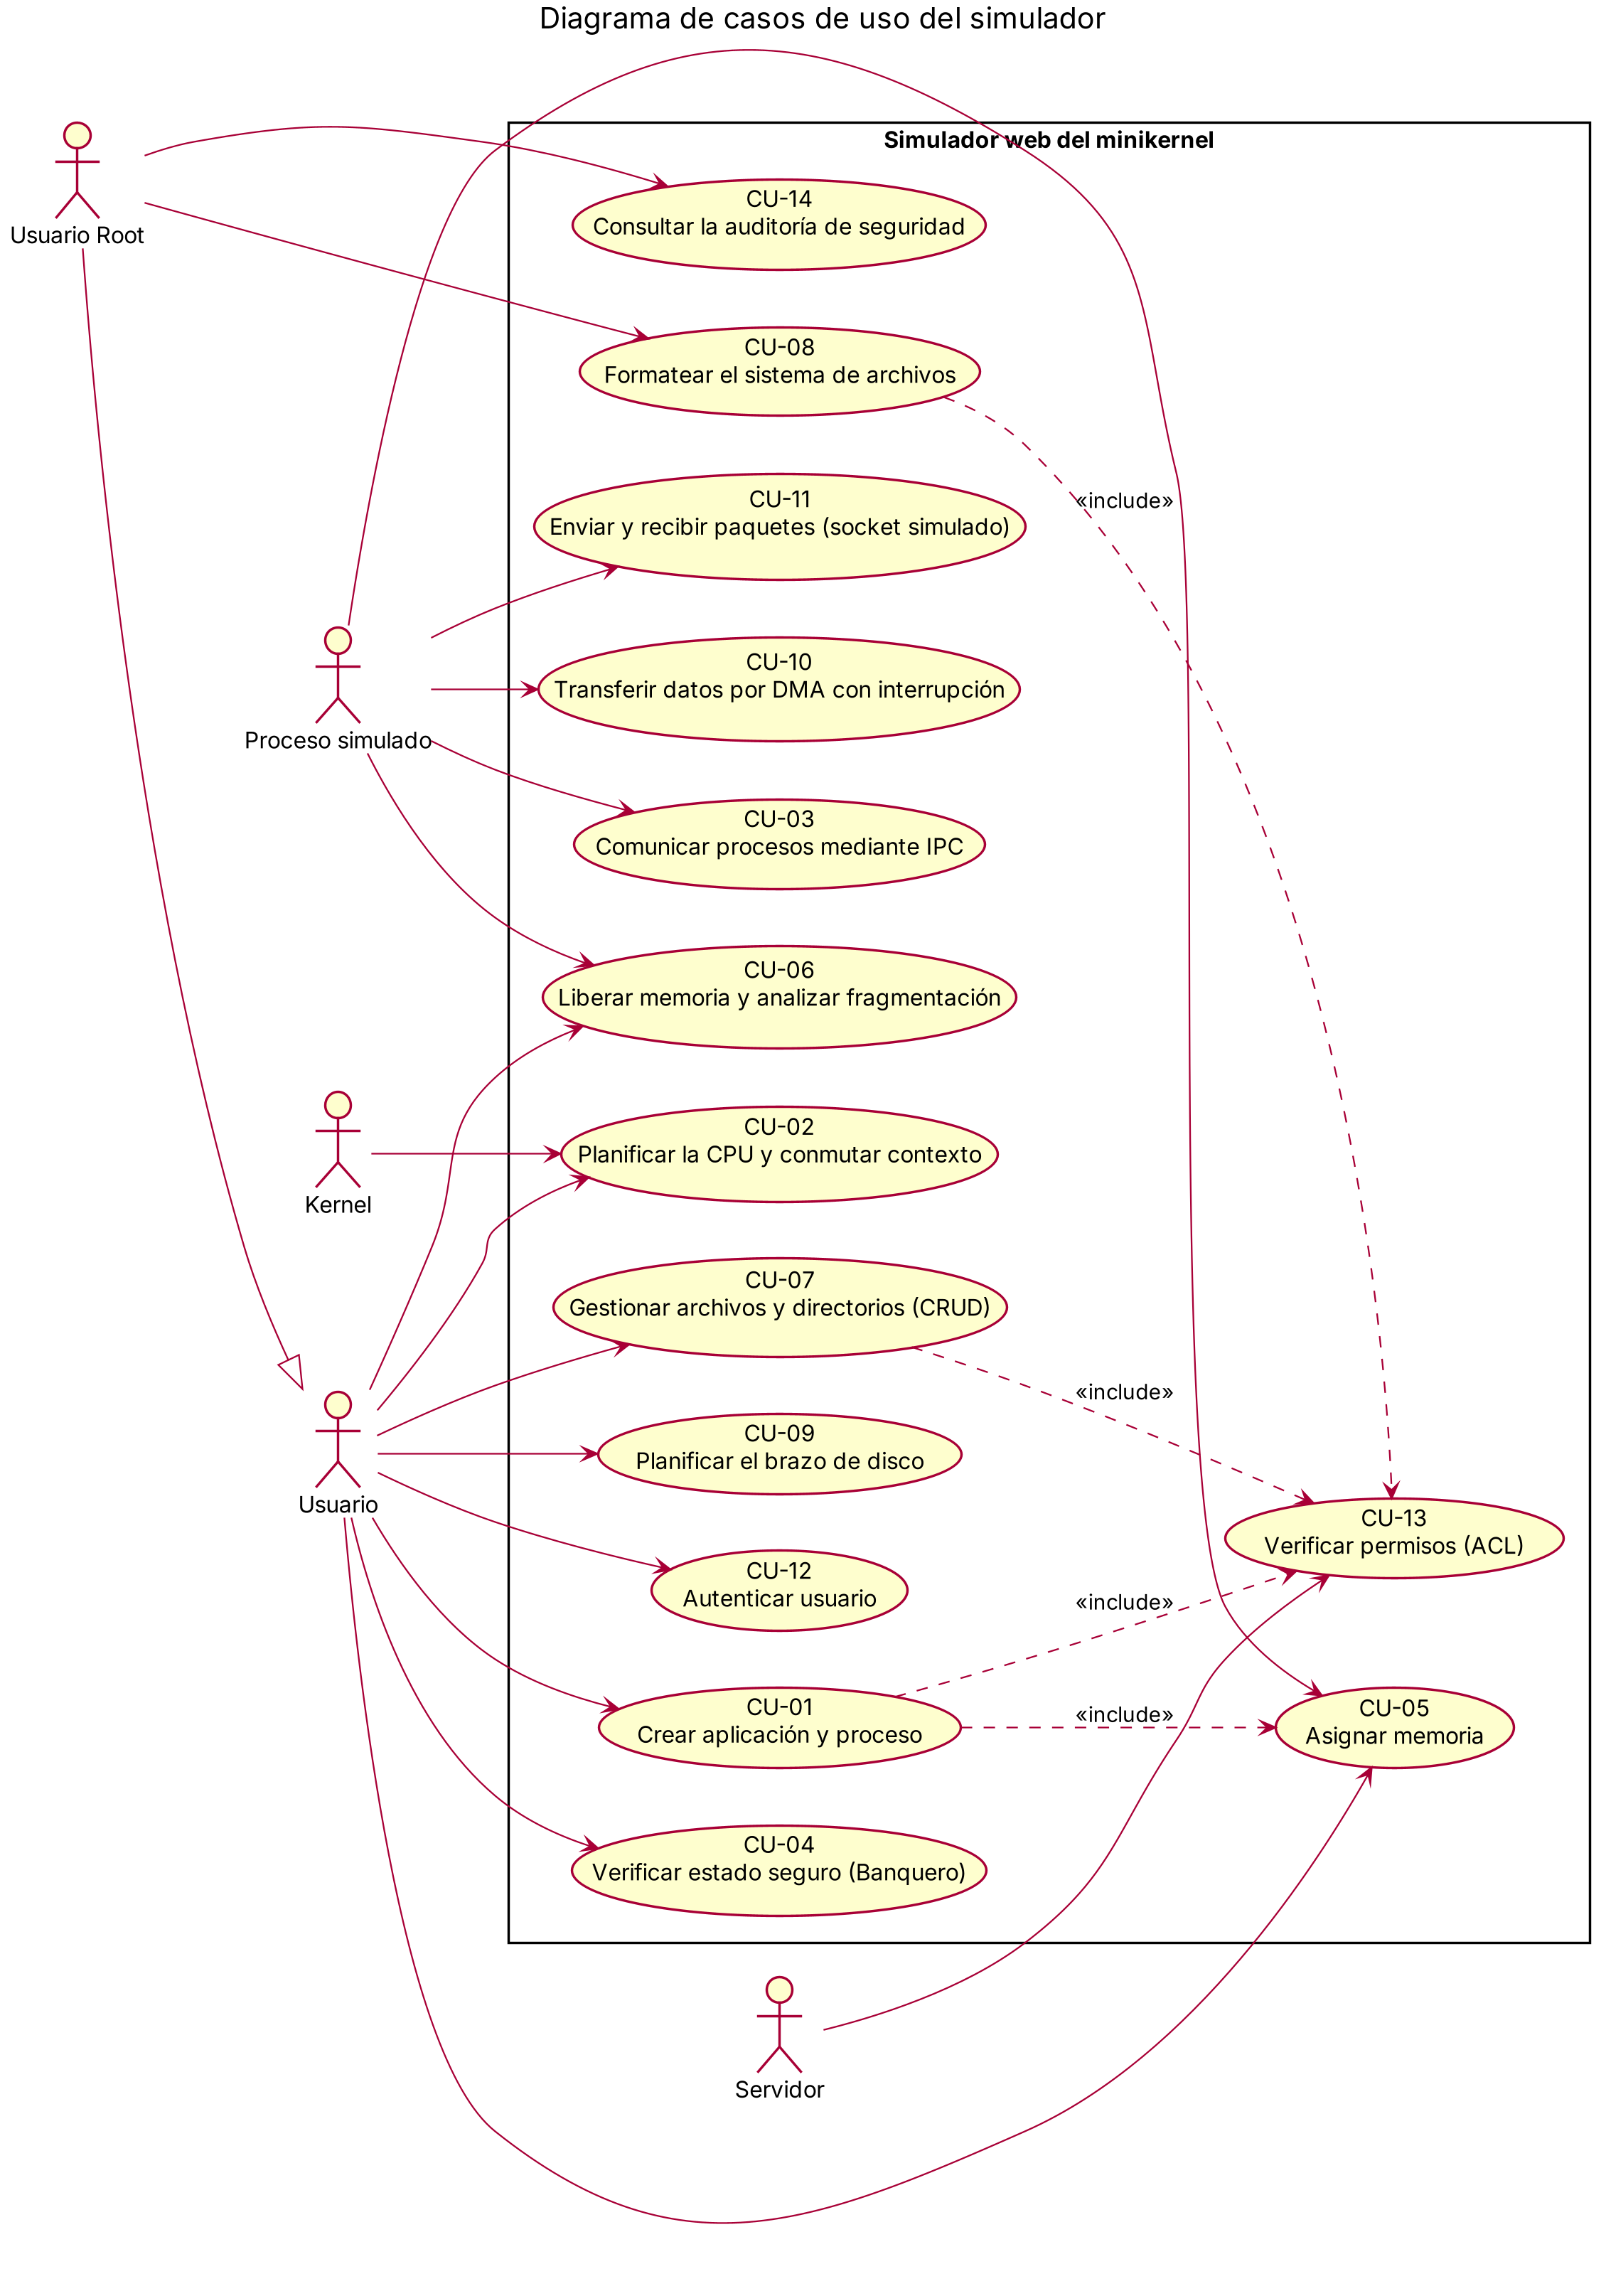
\includegraphics[height=20.5cm,keepaspectratio]{figuras/casos_de_uso.png}
\caption{Diagrama de casos de uso UML del simulador.}
\label{fig:cu}
\end{figure*}

\clearpage
\section{Diagramas de actividad}\label{ax:act}
Las Figs.~\ref{fig:act-cu01} a~\ref{fig:act-cu14} presentan, de forma individual, el diagrama de actividad de cada caso de uso (Sección~\ref{sec:act}).

\begin{figure}[H]
\centering
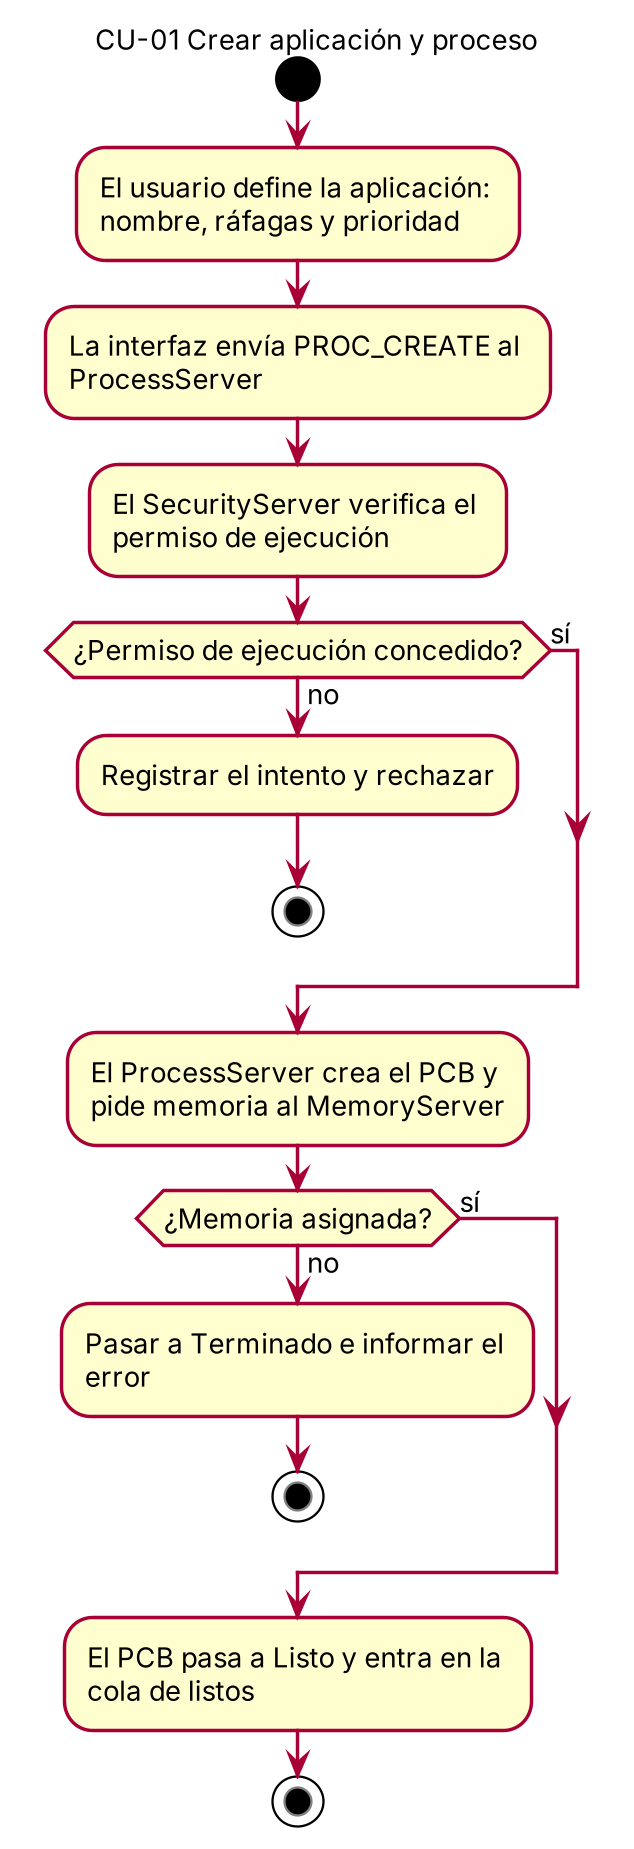
\includegraphics[height=14.09cm,keepaspectratio]{figuras/act_cu01.png}
\caption{Diagrama de actividad UML de CU-01: Crear aplicación y proceso.}
\label{fig:act-cu01}
\end{figure}

\begin{figure}[H]
\centering
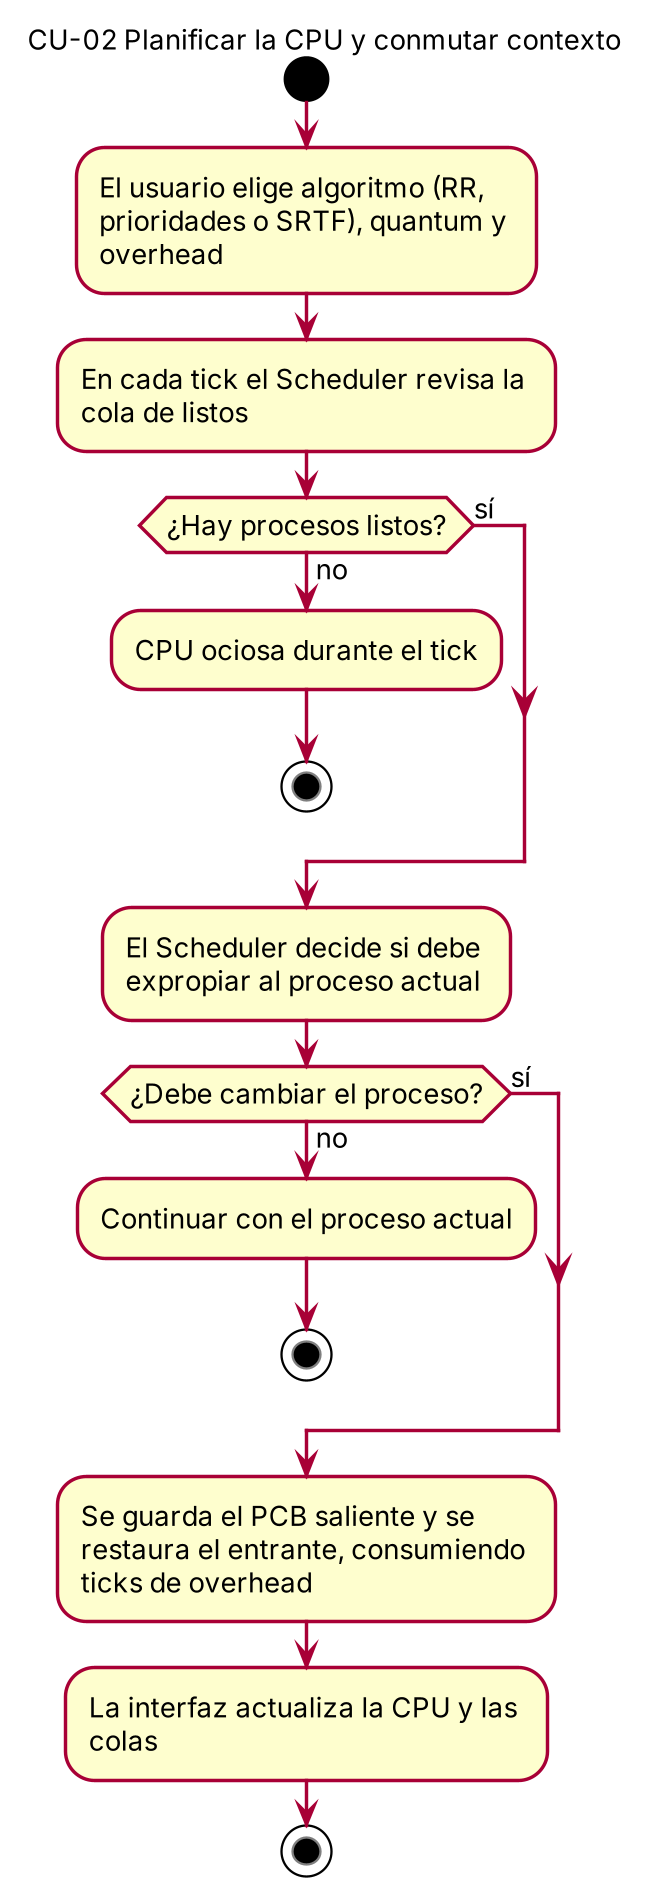
\includegraphics[height=14.47cm,keepaspectratio]{figuras/act_cu02.png}
\caption{Diagrama de actividad UML de CU-02: Planificar la CPU y conmutar contexto.}
\label{fig:act-cu02}
\end{figure}

\begin{figure}[H]
\centering
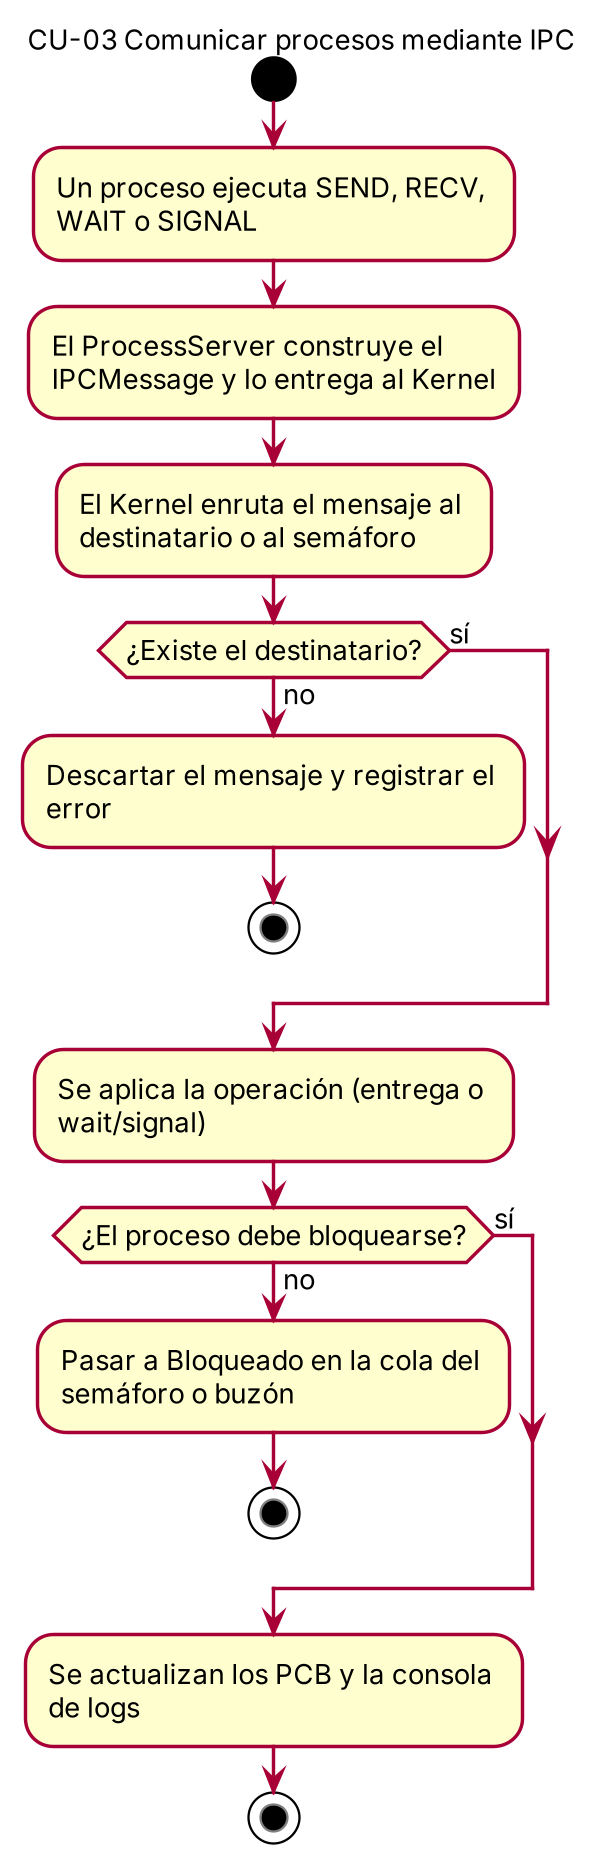
\includegraphics[height=14.22cm,keepaspectratio]{figuras/act_cu03.png}
\caption{Diagrama de actividad UML de CU-03: Comunicar procesos mediante IPC.}
\label{fig:act-cu03}
\end{figure}

\begin{figure}[H]
\centering
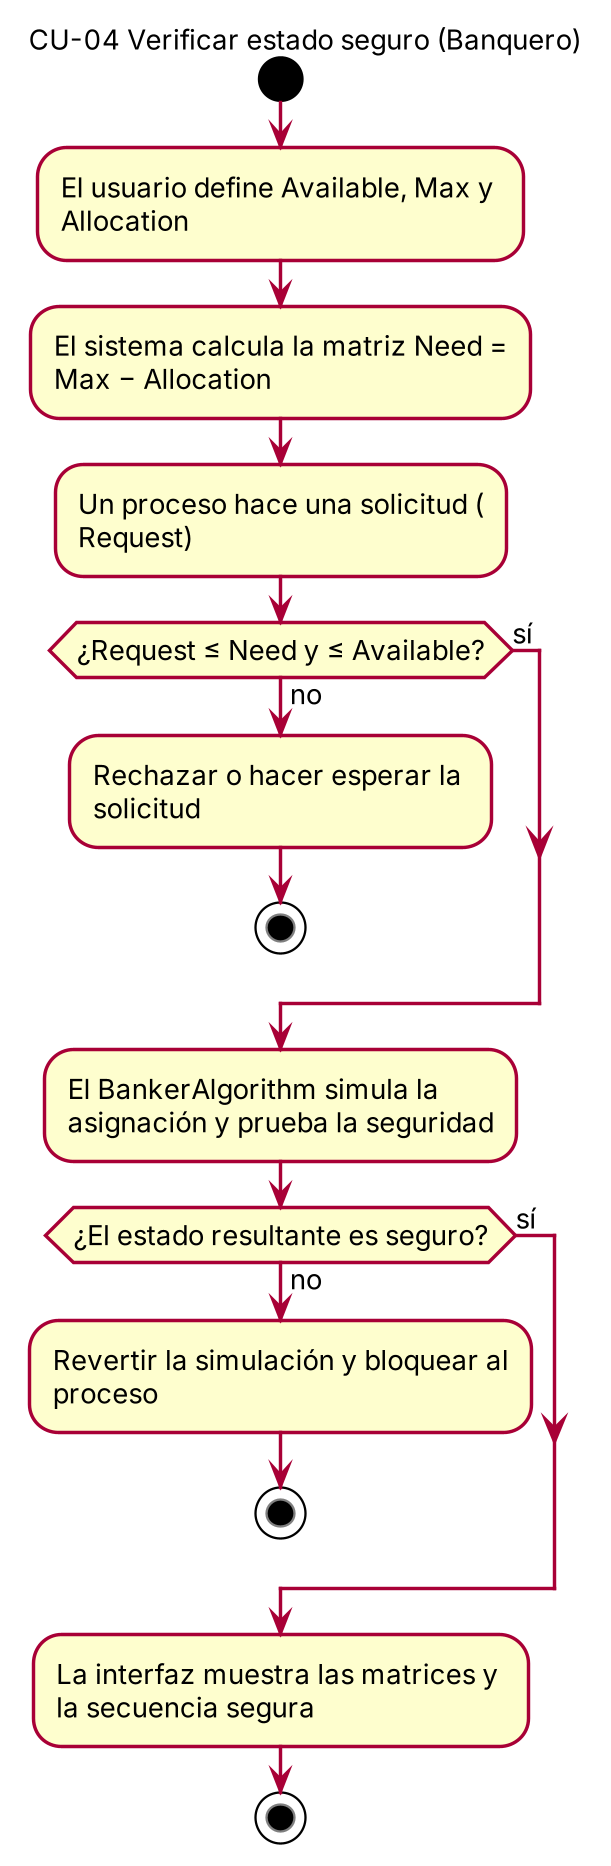
\includegraphics[height=14.22cm,keepaspectratio]{figuras/act_cu04.png}
\caption{Diagrama de actividad UML de CU-04: Verificar estado seguro (Banquero).}
\label{fig:act-cu04}
\end{figure}

\begin{figure}[H]
\centering
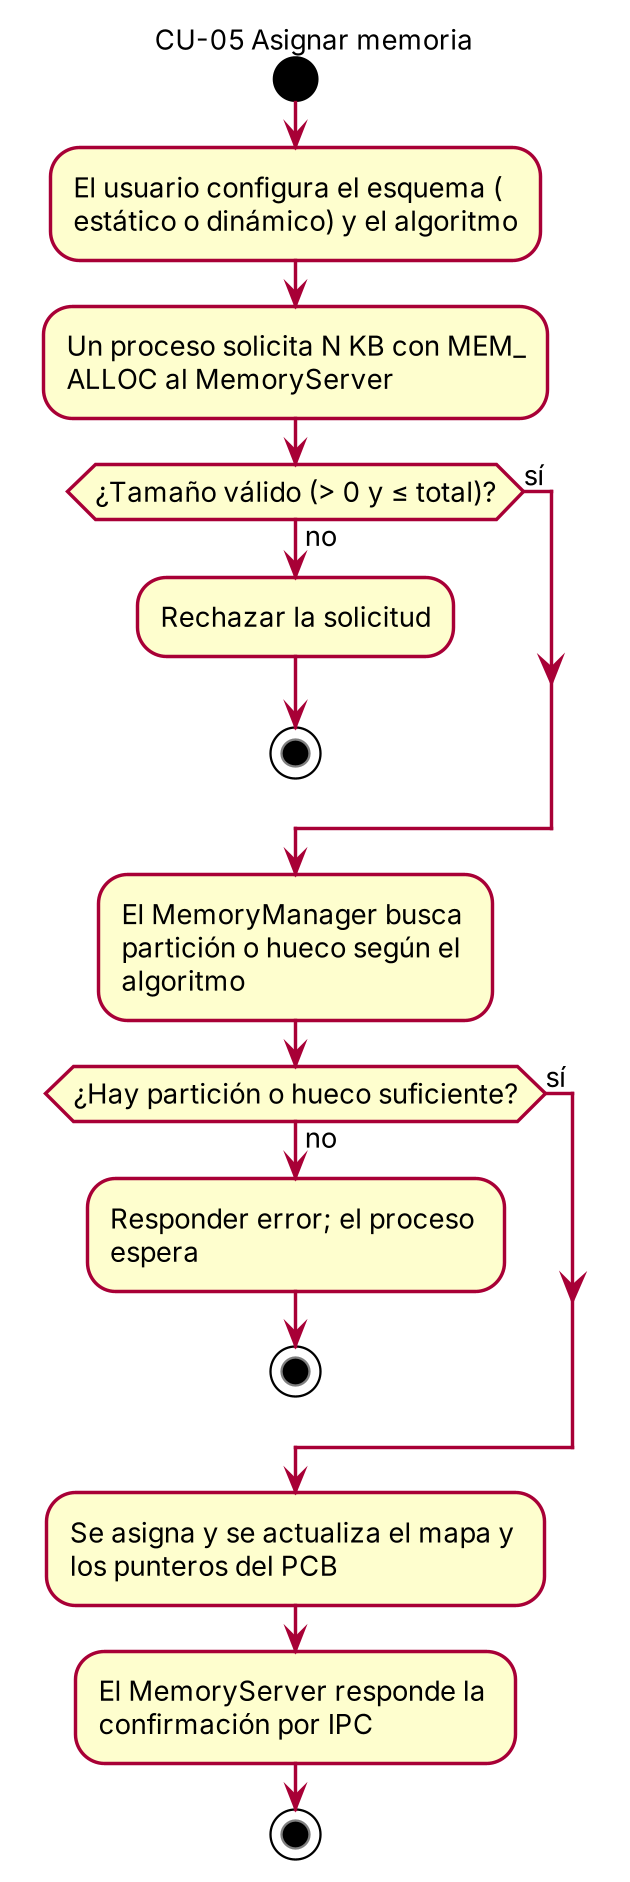
\includegraphics[height=14.34cm,keepaspectratio]{figuras/act_cu05.png}
\caption{Diagrama de actividad UML de CU-05: Asignar memoria.}
\label{fig:act-cu05}
\end{figure}

\begin{figure}[H]
\centering
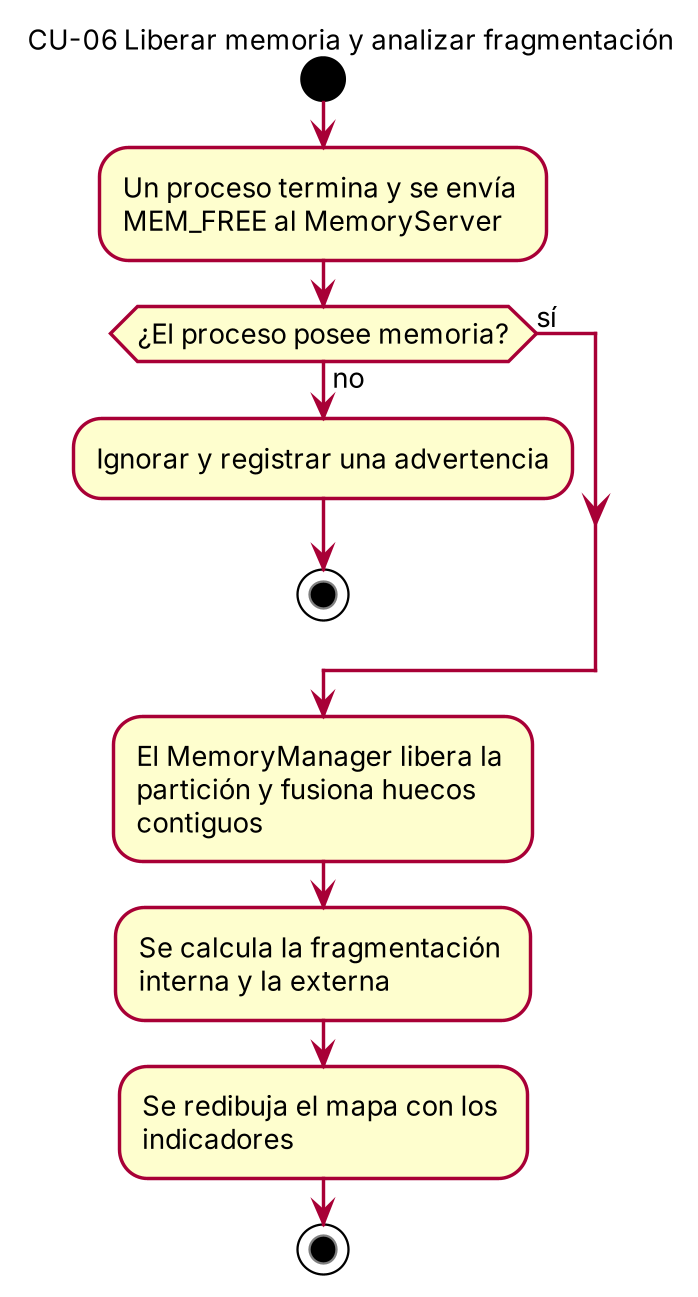
\includegraphics[height=9.88cm,keepaspectratio]{figuras/act_cu06.png}
\caption{Diagrama de actividad UML de CU-06: Liberar memoria y analizar fragmentación.}
\label{fig:act-cu06}
\end{figure}

\begin{figure}[H]
\centering
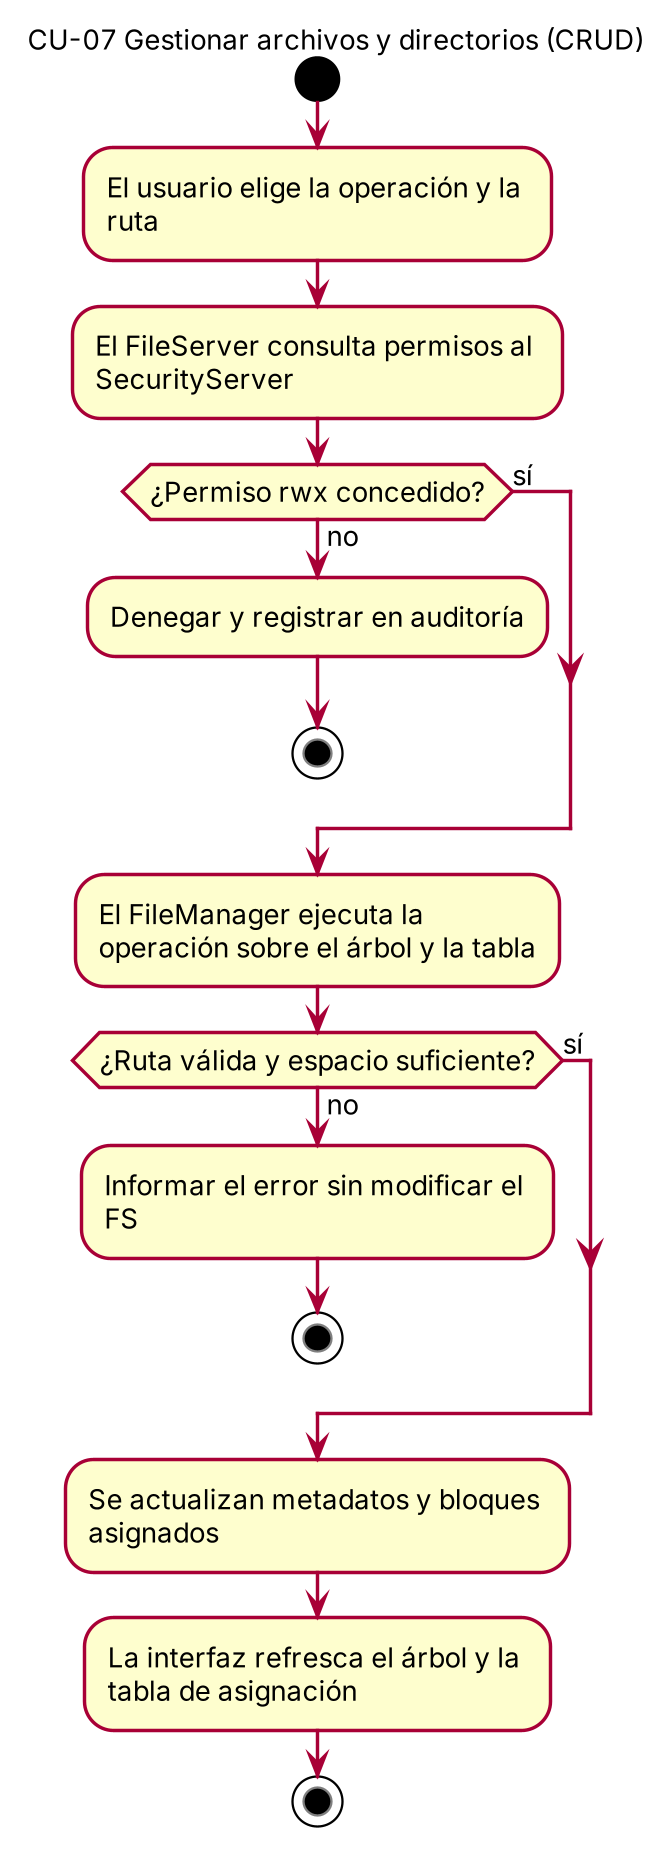
\includegraphics[height=14.09cm,keepaspectratio]{figuras/act_cu07.png}
\caption{Diagrama de actividad UML de CU-07: Gestionar archivos y directorios (CRUD).}
\label{fig:act-cu07}
\end{figure}

\begin{figure}[H]
\centering
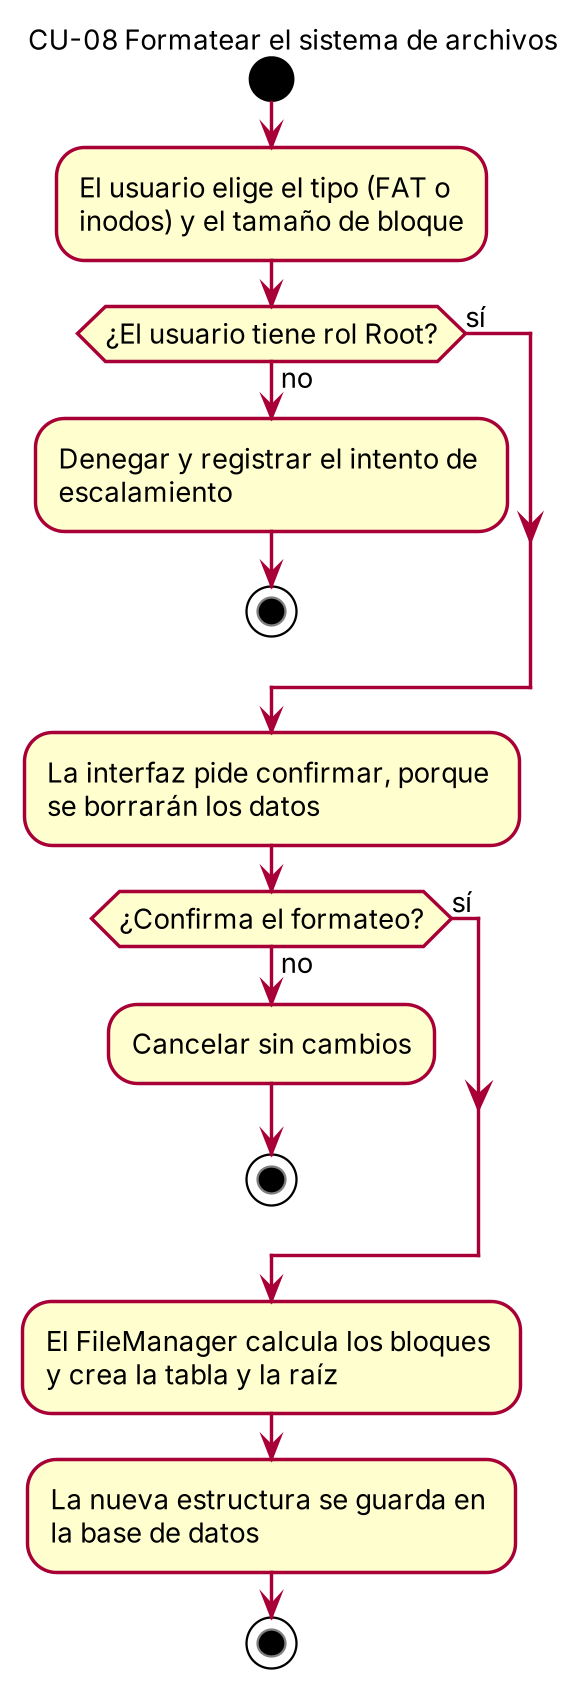
\includegraphics[height=12.89cm,keepaspectratio]{figuras/act_cu08.png}
\caption{Diagrama de actividad UML de CU-08: Formatear el sistema de archivos.}
\label{fig:act-cu08}
\end{figure}

\begin{figure}[H]
\centering
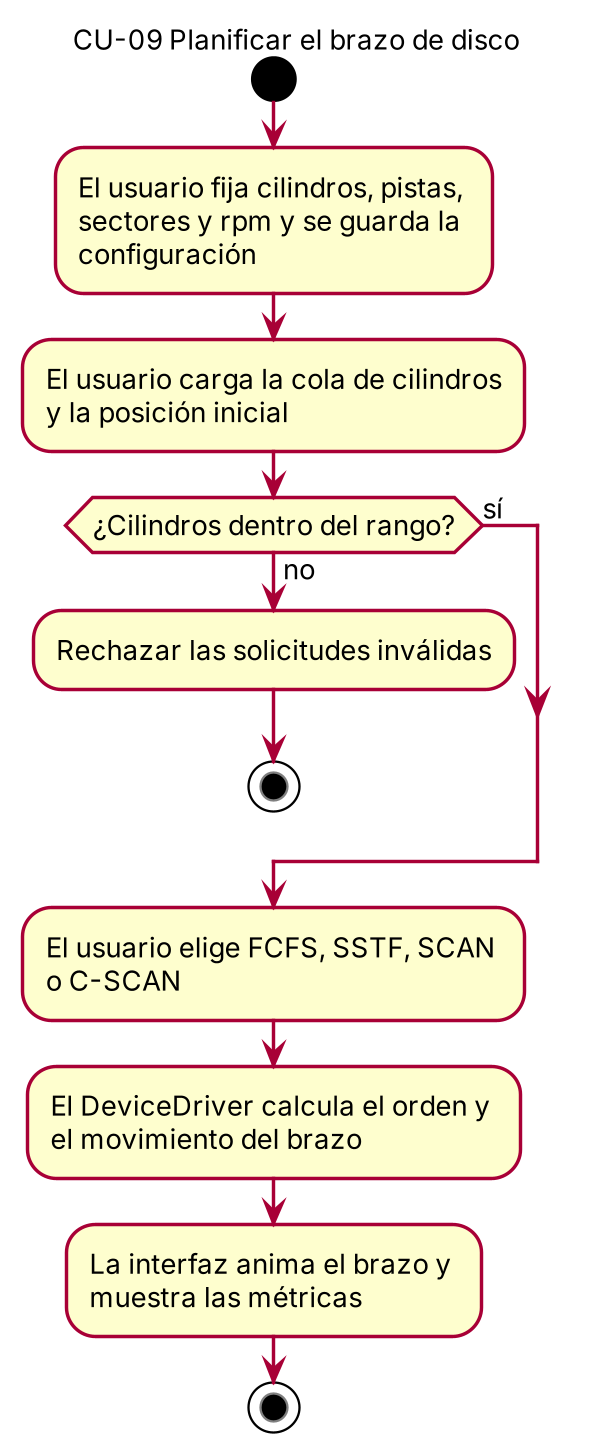
\includegraphics[height=11.09cm,keepaspectratio]{figuras/act_cu09.png}
\caption{Diagrama de actividad UML de CU-09: Planificar el brazo de disco.}
\label{fig:act-cu09}
\end{figure}

\begin{figure}[H]
\centering
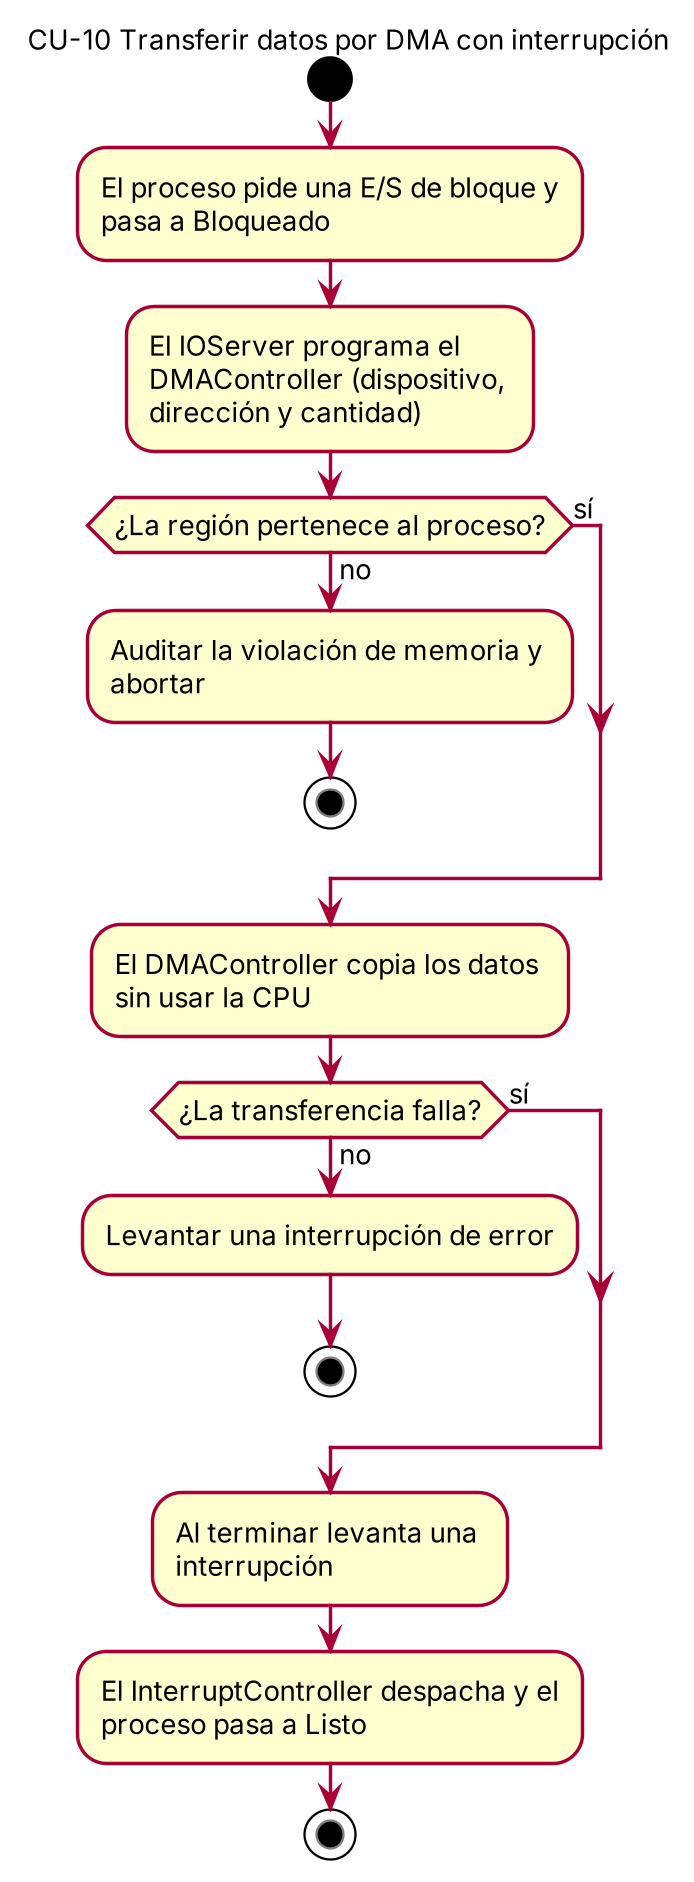
\includegraphics[height=14.34cm,keepaspectratio]{figuras/act_cu10.png}
\caption{Diagrama de actividad UML de CU-10: Transferir datos por DMA con interrupción.}
\label{fig:act-cu10}
\end{figure}

\begin{figure}[H]
\centering
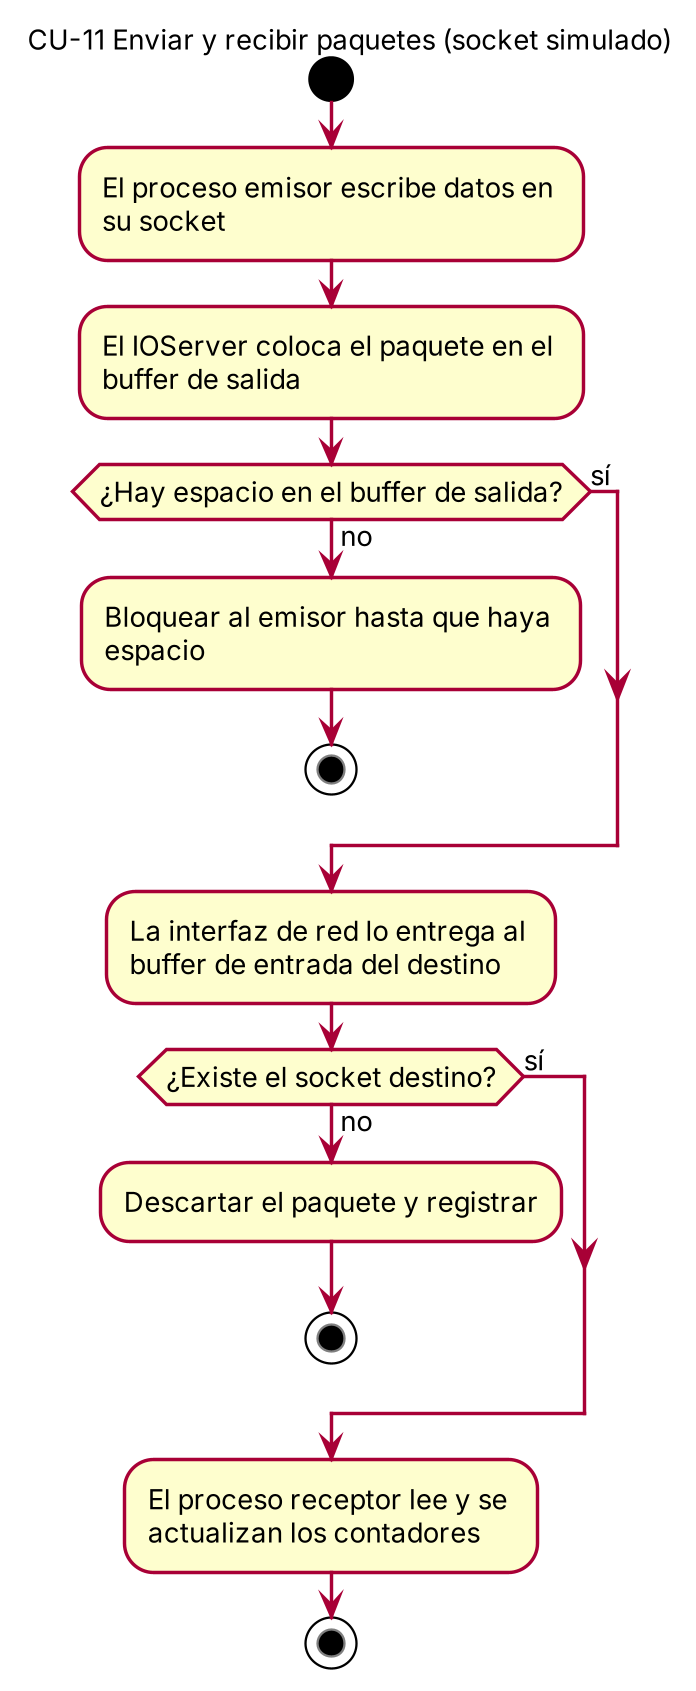
\includegraphics[height=12.89cm,keepaspectratio]{figuras/act_cu11.png}
\caption{Diagrama de actividad UML de CU-11: Enviar y recibir paquetes (socket simulado).}
\label{fig:act-cu11}
\end{figure}

\begin{figure}[H]
\centering
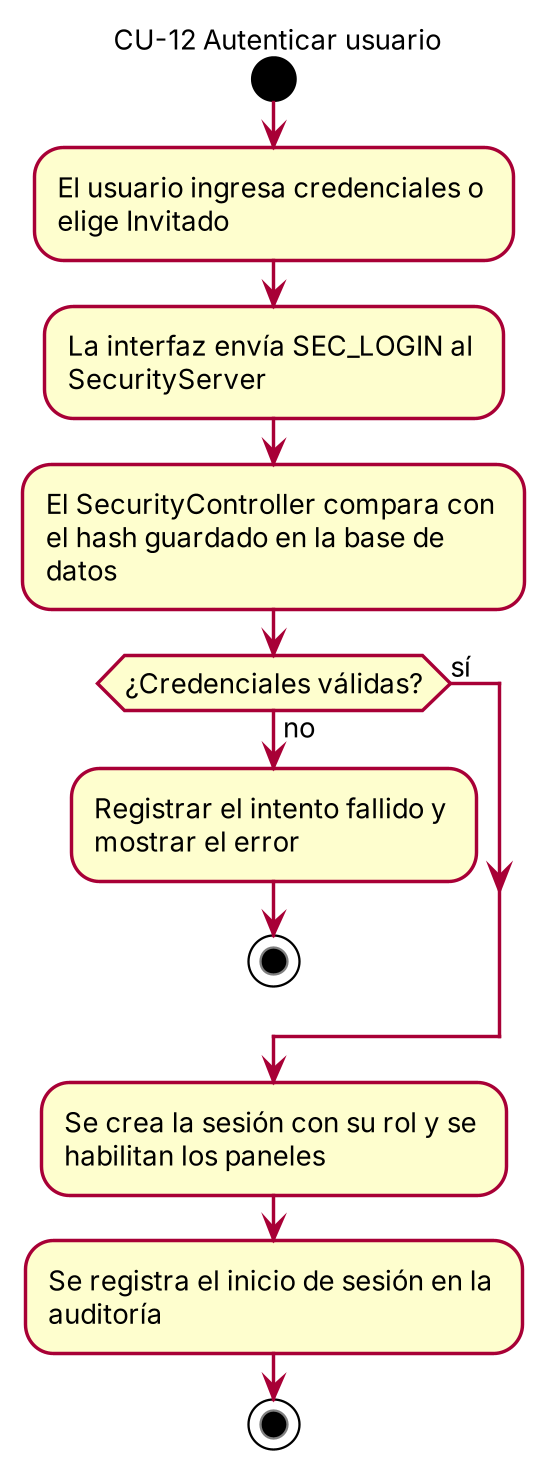
\includegraphics[height=11.22cm,keepaspectratio]{figuras/act_cu12.png}
\caption{Diagrama de actividad UML de CU-12: Autenticar usuario.}
\label{fig:act-cu12}
\end{figure}

\begin{figure}[H]
\centering
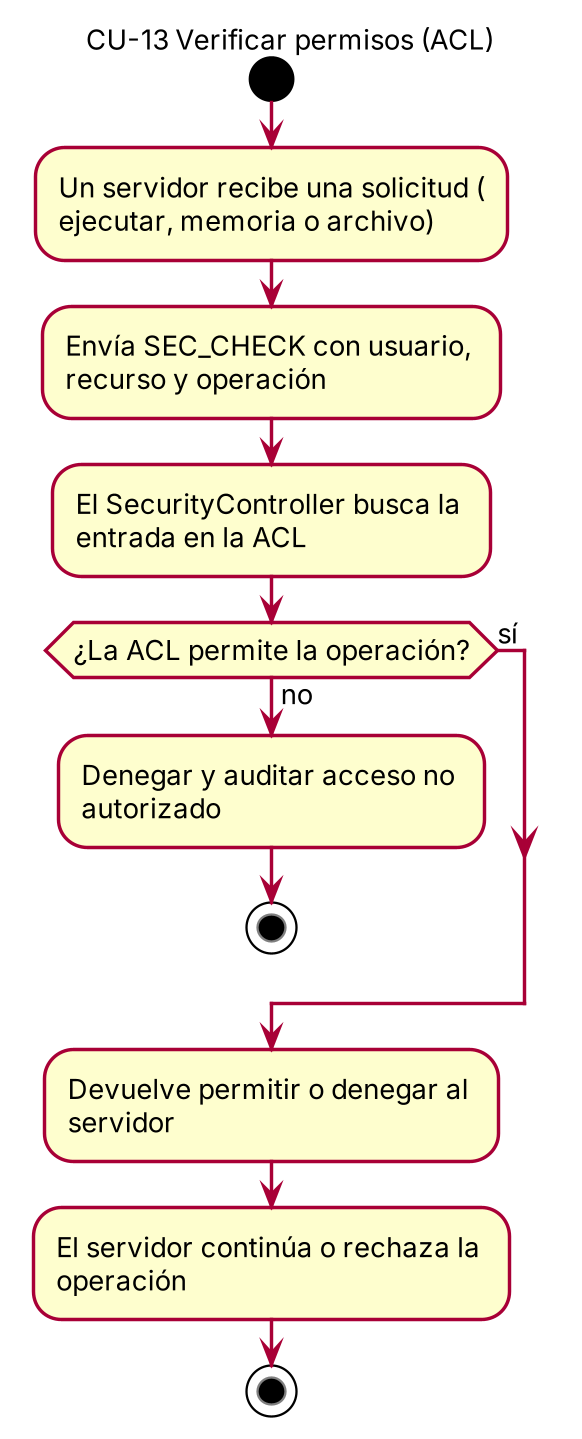
\includegraphics[height=10.97cm,keepaspectratio]{figuras/act_cu13.png}
\caption{Diagrama de actividad UML de CU-13: Verificar permisos (ACL).}
\label{fig:act-cu13}
\end{figure}

\begin{figure}[H]
\centering
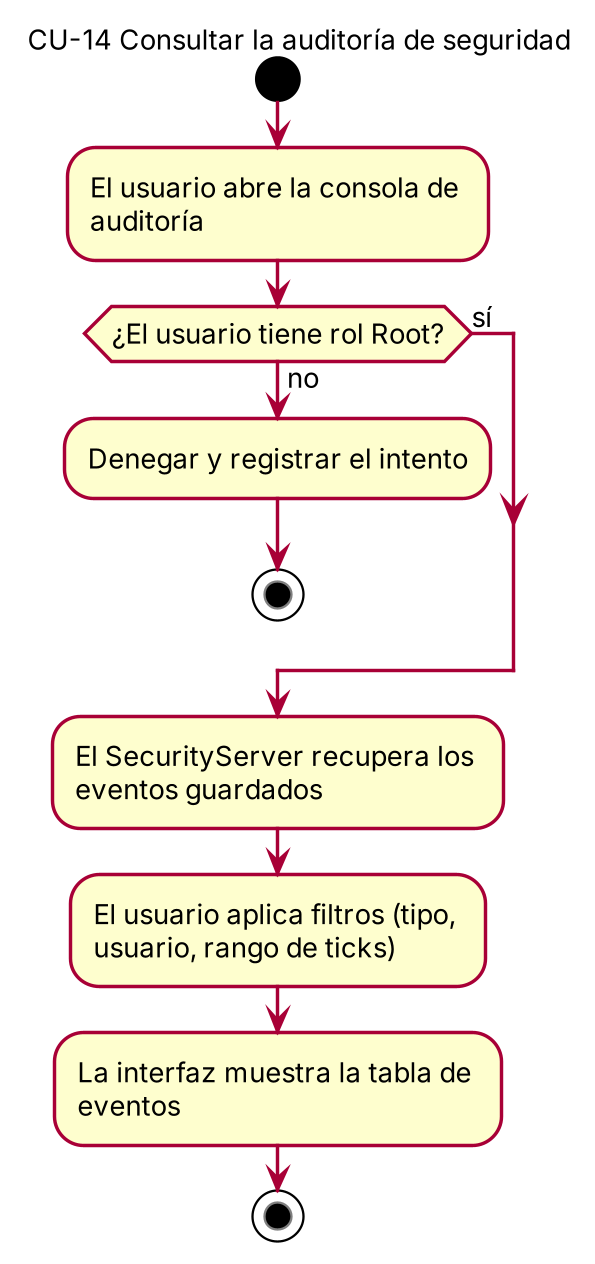
\includegraphics[height=9.63cm,keepaspectratio]{figuras/act_cu14.png}
\caption{Diagrama de actividad UML de CU-14: Consultar la auditoría de seguridad.}
\label{fig:act-cu14}
\end{figure}

\section{Diagrama de clases}\label{ax:cls}
La Fig.~\ref{fig:clases} presenta el modelo de clases descrito en la Sección~\ref{sec:clases}.

\begin{figure*}[!p]
\centering
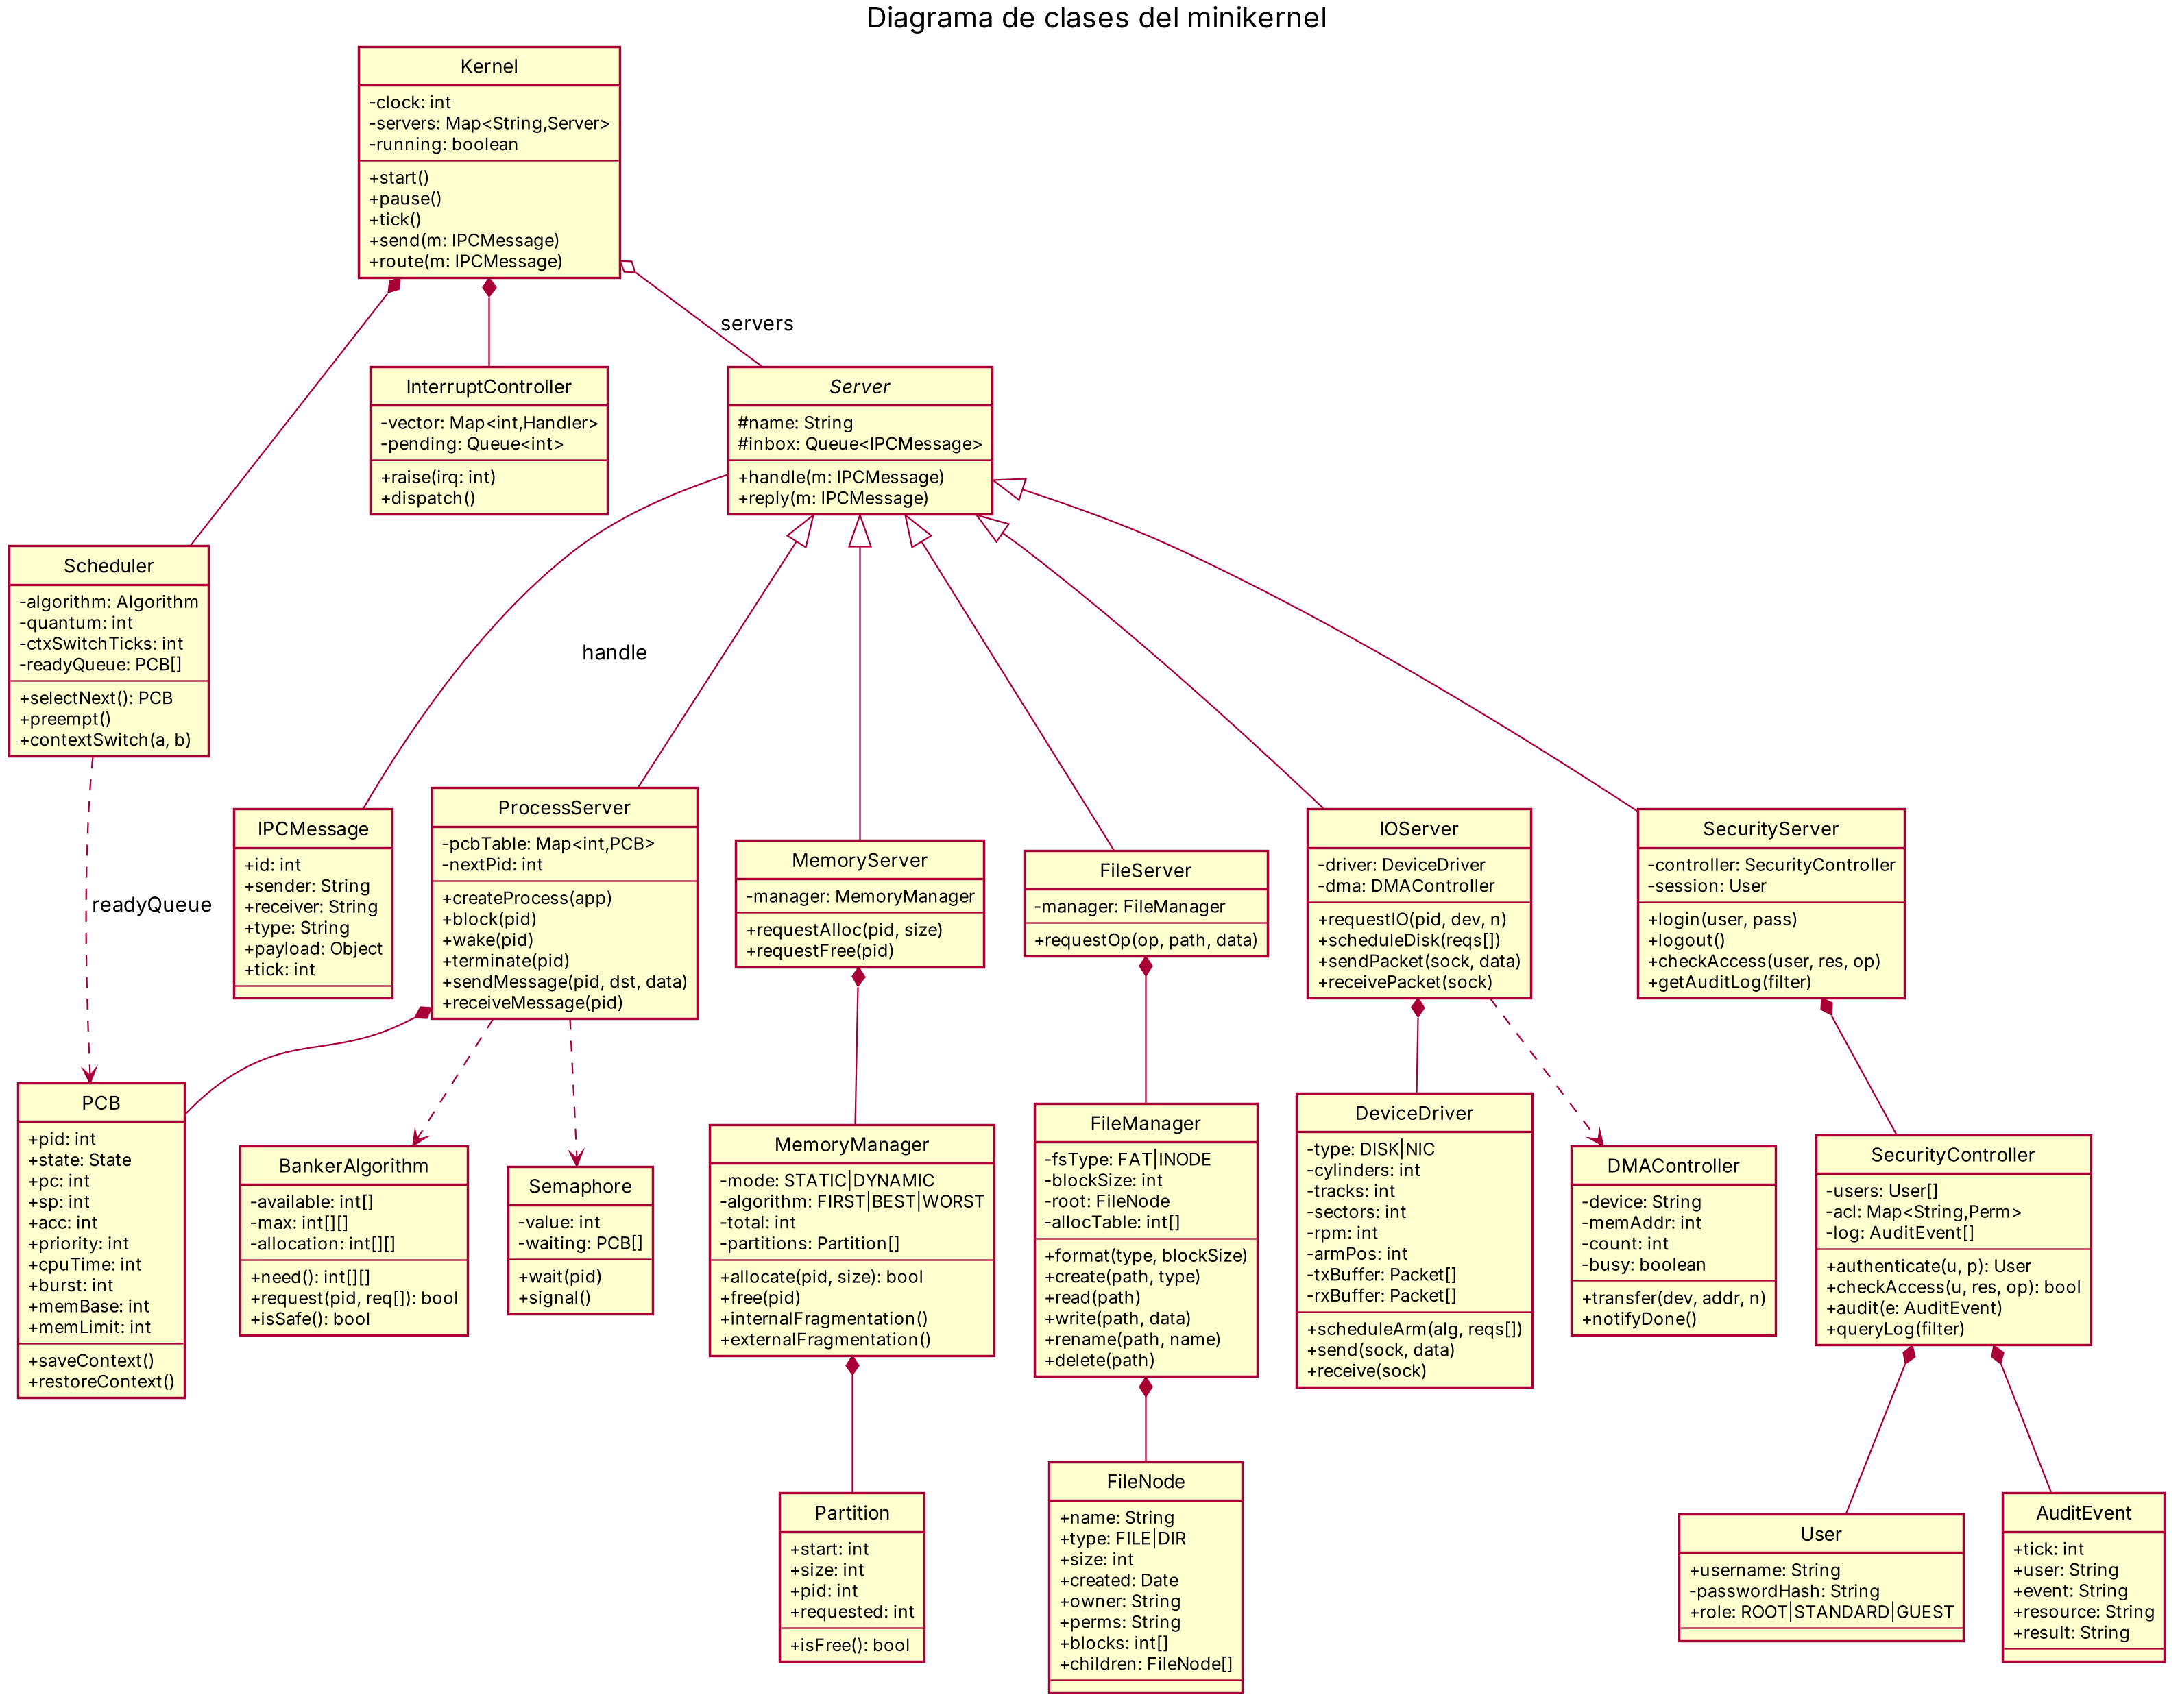
\includegraphics[width=\textwidth,height=21cm,keepaspectratio]{figuras/clases.png}
\caption{Diagrama de clases UML del minikernel.}
\label{fig:clases}
\end{figure*}

\clearpage
\section{Requerimientos funcionales}\label{ax:rf}
Las Tablas~\ref{tab:rf-procesos} a~\ref{tab:rf-nucleo} detallan los requerimientos funcionales por módulo.

\begin{table*}[!t]
\caption{Requerimientos funcionales: Administración de Procesos}
\label{tab:rf-procesos}
\footnotesize\renewcommand{\arraystretch}{1.1}\setlength{\tabcolsep}{2pt}
\begin{tabular}{|>{\raggedright\arraybackslash}p{0.95cm}|>{\raggedright\arraybackslash}p{2.3cm}|>{\raggedright\arraybackslash}p{3.2cm}|>{\raggedright\arraybackslash}p{3.9cm}|>{\raggedright\arraybackslash}p{2.8cm}|>{\raggedright\arraybackslash}p{2.8cm}|>{\raggedright\arraybackslash}p{0.95cm}|}
\hline
\textbf{ID} & \textbf{Nombre} & \textbf{Entrada} & \textbf{Procesamiento} & \textbf{Salida} & \textbf{Restricciones} & \textbf{CU}\\ \hline
RF-01 & Gestión de aplicaciones y procesos & Nombre de la aplicación, lista de ráfagas (CPU/E-S) y prioridad & Registra la aplicación, crea el proceso con PID único y su PCB en estado Nuevo & Proceso visible en la tabla de procesos & Máx. 20 procesos simultáneos; la creación la realiza el ProcessServer & 01\\ \hline
RF-02 & Planificación Round Robin & Quantum en ticks (configurable) & Asigna la CPU por turnos; al agotarse el quantum expropia y reencola & Diagrama de ejecución y métricas de espera y retorno & Quantum \textgreater{}= 1 tick & 02\\ \hline
RF-03 & Prioridades apropiativas & Prioridad de cada PCB & Expropia al proceso en CPU cuando llega uno de mayor prioridad & Orden de ejecución y métricas & Prioridad 0–9; el número menor es la mayor prioridad & 02\\ \hline
RF-04 & Planificación SJF/SRTF & Ráfaga restante de cada proceso & Elige el menor tiempo restante; SRTF expropia al llegar uno más corto & Orden de ejecución y métricas & Las ráfagas se conocen al crear el proceso & 02\\ \hline
RF-05 & Visualización del PCB & Proceso seleccionado & Muestra PID, estado, registros PC, SP y Acc, prioridad, tiempo de CPU y punteros a memoria & Panel del PCB actualizado en cada tick & Estados: Nuevo, Listo, Ejecución, Bloqueado y Terminado & 01, 02\\ \hline
RF-06 & Colas de procesos en tiempo real & Eventos de transición de estado & Mueve el PCB entre la cola de listos, la CPU y las colas de espera de E/S o eventos & Vista gráfica de las colas & Refresco de la interfaz \textless{}= 100 ms & 02\\ \hline
RF-07 & IPC por mensajes y semáforos & Instrucciones SEND, RECV, WAIT y SIGNAL de los procesos & Entrega mensajes o aplica wait/signal; bloquea o despierta procesos & Estado de buzones y semáforos & Toda comunicación pasa por el Kernel & 03\\ \hline
RF-08 & Algoritmo del Banquero & Available, Max, Allocation y solicitud (Request) & Calcula Need = Max - Allocation y ejecuta la prueba de estado seguro & Matrices Allocation, Max y Need; secuencia segura; solicitud concedida o rechazada & Hasta 5 tipos de recurso y 10 procesos & 04\\ \hline
RF-09 & Cambio de contexto con overhead & Ticks de overhead (configurable) & Guarda y restaura el PCB consumiendo ticks sin trabajo útil & Contadores de conmutaciones y de ticks de overhead & Overhead \textgreater{}= 0 ticks & 02\\ \hline
\end{tabular}
\end{table*}

\begin{table*}[!t]
\caption{Requerimientos funcionales: Administración de Memoria}
\label{tab:rf-memoria}
\footnotesize\renewcommand{\arraystretch}{1.1}\setlength{\tabcolsep}{2pt}
\begin{tabular}{|>{\raggedright\arraybackslash}p{0.95cm}|>{\raggedright\arraybackslash}p{2.3cm}|>{\raggedright\arraybackslash}p{3.2cm}|>{\raggedright\arraybackslash}p{3.9cm}|>{\raggedright\arraybackslash}p{2.8cm}|>{\raggedright\arraybackslash}p{2.8cm}|>{\raggedright\arraybackslash}p{0.95cm}|}
\hline
\textbf{ID} & \textbf{Nombre} & \textbf{Entrada} & \textbf{Procesamiento} & \textbf{Salida} & \textbf{Restricciones} & \textbf{CU}\\ \hline
RF-10 & Memoria estática (particiones fijas) & Número y tamaño de las particiones & Asigna un proceso por partición y calcula el espacio desperdiciado & Mapa de particiones & Se configura antes de iniciar la simulación & 05\\ \hline
RF-11 & Memoria dinámica (particiones variables) & Algoritmo (First, Best o Worst-Fit) y tamaño solicitado & Busca un hueco, lo divide y asigna; al liberar fusiona huecos contiguos & Mapa de memoria actualizado & Memoria total configurable (1024 KB por defecto) & 05, 06\\ \hline
RF-12 & Análisis de fragmentación & Estado actual de la memoria & Calcula la fragmentación interna y la externa tras cada asignación o liberación & Valores en KB y \% y mapa con colores & Se recalcula después de cada operación & 06\\ \hline
RF-13 & Servidor de Memoria por mensajes & Solicitudes de asignación y liberación de los procesos & El Kernel enruta el IPCMessage al MemoryServer, que responde & Respuesta de éxito o error & Ningún módulo invoca a MemoryManager directamente & 05, 06\\ \hline
\end{tabular}
\end{table*}

\begin{table*}[!t]
\caption{Requerimientos funcionales: Administración de Archivos}
\label{tab:rf-archivos}
\footnotesize\renewcommand{\arraystretch}{1.1}\setlength{\tabcolsep}{2pt}
\begin{tabular}{|>{\raggedright\arraybackslash}p{0.95cm}|>{\raggedright\arraybackslash}p{2.3cm}|>{\raggedright\arraybackslash}p{3.2cm}|>{\raggedright\arraybackslash}p{3.9cm}|>{\raggedright\arraybackslash}p{2.8cm}|>{\raggedright\arraybackslash}p{2.8cm}|>{\raggedright\arraybackslash}p{0.95cm}|}
\hline
\textbf{ID} & \textbf{Nombre} & \textbf{Entrada} & \textbf{Procesamiento} & \textbf{Salida} & \textbf{Restricciones} & \textbf{CU}\\ \hline
RF-14 & Sistema de archivos jerárquico & Estructura de directorios y archivos & Mantiene el árbol con tamaño, fecha de creación, propietario y permisos rwx & Vista en árbol con metadatos & Nombre único dentro de cada directorio & 07\\ \hline
RF-15 & Formateo FAT o inodos & Tipo de FS y tamaño de bloque o clúster & Construye la tabla FAT o de inodos y el directorio raíz & Estadísticas del FS formateado & Solo Root; el formateo borra los datos & 08\\ \hline
RF-16 & Operaciones CRUD & Operación (crear, leer, modificar, renombrar o eliminar) y ruta & Ejecuta la operación y actualiza metadatos y tabla de asignación & Árbol y tabla de asignación actualizados & Requiere el permiso rwx correspondiente & 07\\ \hline
\end{tabular}
\end{table*}

\begin{table*}[!t]
\caption{Requerimientos funcionales: Administración de Entrada/Salida}
\label{tab:rf-es}
\footnotesize\renewcommand{\arraystretch}{1.1}\setlength{\tabcolsep}{2pt}
\begin{tabular}{|>{\raggedright\arraybackslash}p{0.95cm}|>{\raggedright\arraybackslash}p{2.3cm}|>{\raggedright\arraybackslash}p{3.2cm}|>{\raggedright\arraybackslash}p{3.9cm}|>{\raggedright\arraybackslash}p{2.8cm}|>{\raggedright\arraybackslash}p{2.8cm}|>{\raggedright\arraybackslash}p{0.95cm}|}
\hline
\textbf{ID} & \textbf{Nombre} & \textbf{Entrada} & \textbf{Procesamiento} & \textbf{Salida} & \textbf{Restricciones} & \textbf{CU}\\ \hline
RF-17 & Parametrización de discos & Cilindros, pistas, sectores, rpm y tipo (magnético o SSD) & Valida y guarda la geometría del disco & Disco configurado & Todos los valores > 0 & 09\\ \hline
RF-18 & Planificación del brazo de disco & Cola de cilindros y posición inicial del brazo & Ordena las solicitudes con FCFS, SSTF, SCAN o C-SCAN & Orden de atención y cilindros recorridos & Cilindros dentro del rango del disco & 09\\ \hline
RF-19 & Interrupciones y DMA & Operación de E/S de bloque de un proceso & El DMA copia entre el dispositivo y la RAM sin la CPU y al final levanta una interrupción & Bitácora de interrupciones y estado del canal DMA & La CPU no participa en la copia & 10\\ \hline
RF-20 & Interfaz de red simulada & Paquete, socket de origen y de destino & Encola el paquete en el buffer de salida y lo entrega al buffer de entrada del destino & Paquetes recibidos y contadores & Buffers de tamaño finito & 11\\ \hline
\end{tabular}
\end{table*}

\begin{table*}[!t]
\caption{Requerimientos funcionales: Administración de Seguridad}
\label{tab:rf-seguridad}
\footnotesize\renewcommand{\arraystretch}{1.1}\setlength{\tabcolsep}{2pt}
\begin{tabular}{|>{\raggedright\arraybackslash}p{0.95cm}|>{\raggedright\arraybackslash}p{2.3cm}|>{\raggedright\arraybackslash}p{3.2cm}|>{\raggedright\arraybackslash}p{3.9cm}|>{\raggedright\arraybackslash}p{2.8cm}|>{\raggedright\arraybackslash}p{2.8cm}|>{\raggedright\arraybackslash}p{0.95cm}|}
\hline
\textbf{ID} & \textbf{Nombre} & \textbf{Entrada} & \textbf{Procesamiento} & \textbf{Salida} & \textbf{Restricciones} & \textbf{CU}\\ \hline
RF-21 & Autenticación y perfiles & Usuario y contraseña, o acceso como Invitado & Valida las credenciales y crea la sesión & Sesión con rol Root, Estándar o Invitado & Contraseñas almacenadas como hash & 12\\ \hline
RF-22 & Control de acceso (ACL) & Usuario, recurso y operación & Consulta la matriz ACL para ejecución de procesos, memoria y archivos & Decisión de permitir o denegar & Toda operación pasa por el SecurityServer & 01, 07, 08, 13\\ \hline
RF-23 & Auditoría de seguridad & Eventos de seguridad & Registra accesos no autorizados, violaciones de memoria y escalamientos de privilegios fallidos & Tabla de eventos filtrable & Solo Root la consulta; el log no se edita & 10, 12, 13, 14\\ \hline
\end{tabular}
\end{table*}

\begin{table*}[!t]
\caption{Requerimientos funcionales: Microkernel y servicios transversales}
\label{tab:rf-nucleo}
\footnotesize\renewcommand{\arraystretch}{1.1}\setlength{\tabcolsep}{2pt}
\begin{tabular}{|>{\raggedright\arraybackslash}p{0.95cm}|>{\raggedright\arraybackslash}p{2.3cm}|>{\raggedright\arraybackslash}p{3.2cm}|>{\raggedright\arraybackslash}p{3.9cm}|>{\raggedright\arraybackslash}p{2.8cm}|>{\raggedright\arraybackslash}p{2.8cm}|>{\raggedright\arraybackslash}p{0.95cm}|}
\hline
\textbf{ID} & \textbf{Nombre} & \textbf{Entrada} & \textbf{Procesamiento} & \textbf{Salida} & \textbf{Restricciones} & \textbf{CU}\\ \hline
RF-24 & Servicios mínimos del microkernel & IPCMessage, interrupciones y ticks de reloj & El Kernel solo planifica, enruta mensajes y despacha interrupciones; lo demás vive en servidores & Mensajes entregados a cada servidor & Los servidores no se invocan entre sí directamente & 01, 03, 05\\ \hline
RF-25 & Reloj de simulación y consola de logs & Controles iniciar, pausar, paso a paso y velocidad & Avanza los ticks y registra los eventos en la consola & Consola de logs & Velocidad configurable & 02, 03\\ \hline
RF-26 & Persistencia local & Usuarios, logs, configuración de discos y sistema de archivos & Guarda y restaura el estado en una base de datos relacional mediante JPA & Estado conservado al recargar la página o reiniciar el servidor & Base H2 o PostgreSQL local; sin servicios externos & 08, 09, 12, 14\\ \hline
\end{tabular}
\end{table*}

\clearpage
\section{Requerimientos no funcionales}\label{ax:rnf}
La Tabla~\ref{tab:rnf} recoge los atributos de calidad y su verificación.

\begin{table*}[!t]
\caption{Requerimientos no funcionales}
\label{tab:rnf}
\footnotesize\renewcommand{\arraystretch}{1.1}\setlength{\tabcolsep}{3pt}
\begin{tabular}{|>{\raggedright\arraybackslash}p{1.2cm}|>{\raggedright\arraybackslash}p{3.0cm}|>{\raggedright\arraybackslash}p{8.2cm}|>{\raggedright\arraybackslash}p{4.6cm}|}
\hline
\textbf{ID} & \textbf{Atributo} & \textbf{Descripción} & \textbf{Verificación}\\ \hline
RNF-01 & Arquitectura microkernel & El núcleo solo ofrece planificación básica, IPC e interrupciones; los cinco servidores se ejecutan aislados y se comunican únicamente con IPCMessage. & Revisión de dependencias: ningún paquete de servidor importa a otro ni se inyecta como bean en otro.\\ \hline
RNF-02 & Plataforma web & Backend en Java 17 con Spring Boot 3 que ejecuta el simulador y cliente web (Thymeleaf y JavaScript) conectado por WebSocket (STOMP) y REST. & El servidor arranca con un solo comando (mvn spring-boot:run) y la interfaz funciona en Chrome, Edge y Firefox recientes.\\ \hline
RNF-03 & Rendimiento & La simulación avanza al menos 10 ticks por segundo y el estado llega a la interfaz en \textless{}= 100 ms (latencia del WebSocket) con 20 procesos. & Medición en la demostración con 20 procesos.\\ \hline
RNF-04 & Reproducibilidad & La misma configuración y la misma semilla producen la misma traza de ejecución. & Dos ejecuciones con igual semilla generan igual registro.\\ \hline
RNF-05 & Usabilidad & Los parámetros se editan en modales con validación y mensajes de error claros, sin escribir código. & Cada parámetro de los RF se puede cambiar desde la interfaz.\\ \hline
RNF-06 & Persistencia & Los datos de RF-26 sobreviven a recargar la página y a reiniciar el servidor, y existe una opción para restablecer la base. & Reiniciar el servidor y comprobar usuarios, logs, discos y FS.\\ \hline
RNF-07 & Seguridad de la simulación & Los programas simulados son listas de instrucciones del propio simulador; no se ejecuta código arbitrario (sin ScriptEngine ni reflexión dinámica). & Revisión del código: no se usa ScriptEngine, reflexión dinámica ni Runtime.exec.\\ \hline
RNF-08 & Mantenibilidad & Un paquete Java por servidor, con la interfaz de mensajes documentada en la tabla de tipos de IPCMessage. & Cada tipo de mensaje tiene un único servidor receptor.\\ \hline
RNF-09 & Coherencia y trazabilidad & Nombres de clases, métodos y tipos de mensaje idénticos en informe, diagramas y código; cada RF tiene al menos un CU. & Matriz de trazabilidad y revisión cruzada antes de cada entrega.\\ \hline
RNF-10 & Aislamiento por sesión & Cada sesión del navegador tiene su propia instancia del Kernel y de los servidores; dos usuarios no comparten ticks ni procesos. & Abrir dos pestañas y comprobar que la simulación es independiente.\\ \hline
\end{tabular}
\end{table*}

\section{Tipos de mensaje IPC}\label{ax:msg}
La Tabla~\ref{tab:msg} define los tipos de \texttt{IPCMessage} y el servidor que los recibe.

\begin{table}[!t]
\caption{Tipos de IPCMessage y servidor receptor}
\label{tab:msg}
\scriptsize\renewcommand{\arraystretch}{1.1}\setlength{\tabcolsep}{2pt}
\begin{tabular}{|>{\raggedright\arraybackslash}p{2.5cm}|>{\raggedright\arraybackslash}p{2.9cm}|>{\raggedright\arraybackslash}p{2.9cm}|}
\hline \textbf{Tipo} & \textbf{Emisor \textrightarrow{} receptor} & \textbf{Propósito}\\ \hline
\texttt{PROC\_CREATE} & UI \textrightarrow{} ProcessServer & Crear aplicación y proceso\\ \hline
\texttt{IPC\_SEND/\allowbreak IPC\_RECV} & Proceso \textrightarrow{} ProcessServer & Enviar o recibir un mensaje entre procesos\\ \hline
\texttt{SEM\_WAIT/\allowbreak SEM\_SIGNAL} & Proceso \textrightarrow{} ProcessServer & Operaciones sobre semáforos\\ \hline
\texttt{MEM\_ALLOC/\allowbreak MEM\_FREE} & ProcessServer \textrightarrow{} MemoryServer & Asignar o liberar memoria\\ \hline
\texttt{FS\_OP} & UI \textrightarrow{} FileServer & Crear, leer, modificar, renombrar, eliminar o formatear\\ \hline
\texttt{IO\_DISK} & UI \textrightarrow{} IOServer & Planificar el brazo de disco\\ \hline
\texttt{IO\_DMA} & ProcessServer \textrightarrow{} IOServer & Programar una transferencia DMA\\ \hline
\texttt{NET\_SEND/\allowbreak NET\_RECV} & Proceso \textrightarrow{} IOServer & Enviar o recibir un paquete por socket\\ \hline
\texttt{SEC\_LOGIN} & UI \textrightarrow{} SecurityServer & Autenticar un usuario\\ \hline
\texttt{SEC\_CHECK} & Cualquier servidor \textrightarrow{} SecurityServer & Consultar la ACL\\ \hline
\texttt{SEC\_AUDIT} & Cualquier servidor \textrightarrow{} SecurityServer & Registrar o consultar eventos de auditoría\\ \hline
\texttt{IRQ\_DONE} & DMAController \textrightarrow{} Kernel & Interrupción de fin de transferencia\\ \hline
\end{tabular}
\end{table}

\clearpage
\section{Especificación de casos de uso}\label{ax:cu}
Las Tablas~\ref{tab:cu1} y~\ref{tab:cu2} especifican los casos de uso.

\begin{table*}[!t]
\caption{Especificación de casos de uso (CU-01 a CU-07)}
\label{tab:cu1}
\scriptsize\renewcommand{\arraystretch}{1.05}\setlength{\tabcolsep}{2pt}
\begin{tabular}{|>{\raggedright}p{0.8cm}|>{\raggedright}p{2.1cm}|>{\raggedright}p{1.7cm}|>{\raggedright}p{4.7cm}|>{\raggedright}p{2.9cm}|>{\raggedright}p{1.8cm}|>{\raggedright}p{2.9cm}|}
\hline
\textbf{ID} & \textbf{Nombre y actor} & \textbf{Precondición} & \textbf{Flujo principal} & \textbf{Flujos alternos} & \textbf{Postcondición} & \textbf{Clases y métodos}\tabularnewline \hline
CU-01 & \textbf{Crear aplicación y proceso}\\ \textit{Procesos}\\ Actor: Usuario & Sesión iniciada con permiso de ejecución & 1. El usuario define la aplicación: nombre, ráfagas y prioridad\\ 2. La interfaz envía PROC\_CREATE al ProcessServer\\ 3. El SecurityServer verifica el permiso de ejecución\\ 4. El ProcessServer crea el PCB y pide memoria al MemoryServer\\ 5. El PCB pasa a Listo y entra en la cola de listos & 3a. ¿Permiso de ejecución concedido?: Registrar el intento y rechazar\\ 4a. ¿Memoria asignada?: Pasar a Terminado e informar el error & PCB visible en la tabla de procesos en estado Listo & ProcessServer.\allowbreak createProcess, SecurityController.\allowbreak checkAccess, MemoryManager.\allowbreak allocate, Kernel.\allowbreak route\tabularnewline \hline
CU-02 & \textbf{Planificar la CPU y conmutar contexto}\\ \textit{Procesos}\\ Actor: Usuario, Kernel & Existe al menos un proceso creado & 1. El usuario elige algoritmo (RR, prioridades o SRTF), quantum y overhead\\ 2. En cada tick el Scheduler revisa la cola de listos\\ 3. El Scheduler decide si debe expropiar al proceso actual\\ 4. Se guarda el PCB saliente y se restaura el entrante, consumiendo ticks de overhead\\ 5. La interfaz actualiza la CPU y las colas & 2a. ¿Hay procesos listos?: CPU ociosa durante el tick\\ 3a. ¿Debe cambiar el proceso?: Continuar con el proceso actual & Un PCB en Ejecución y colas actualizadas & Kernel.\allowbreak tick, Scheduler.\allowbreak selectNext, Scheduler.\allowbreak preempt, Scheduler.\allowbreak contextSwitch, PCB.\allowbreak saveContext, PCB.\allowbreak restoreContext\tabularnewline \hline
CU-03 & \textbf{Comunicar procesos mediante IPC}\\ \textit{Procesos}\\ Actor: Proceso simulado & Dos o más procesos creados & 1. Un proceso ejecuta SEND, RECV, WAIT o SIGNAL\\ 2. El ProcessServer construye el IPCMessage y lo entrega al Kernel\\ 3. El Kernel enruta el mensaje al destinatario o al semáforo\\ 4. Se aplica la operación (entrega o wait/signal)\\ 5. Se actualizan los PCB y la consola de logs & 3a. ¿Existe el destinatario?: Descartar el mensaje y registrar el error\\ 4a. ¿El proceso debe bloquearse?: Pasar a Bloqueado en la cola del semáforo o buzón & Mensaje entregado o proceso bloqueado, con log registrado & ProcessServer.\allowbreak sendMessage, ProcessServer.\allowbreak receiveMessage, Kernel.\allowbreak send, Kernel.\allowbreak route, Semaphore.\allowbreak wait, Semaphore.\allowbreak signal, ProcessServer.\allowbreak block, ProcessServer.\allowbreak wake\tabularnewline \hline
CU-04 & \textbf{Verificar estado seguro (Banquero)}\\ \textit{Procesos}\\ Actor: Usuario & Recursos y procesos configurados & 1. El usuario define Available, Max y Allocation\\ 2. El sistema calcula la matriz Need = Max - Allocation\\ 3. Un proceso hace una solicitud (Request)\\ 4. El BankerAlgorithm simula la asignación y prueba la seguridad\\ 5. La interfaz muestra las matrices y la secuencia segura & 3a. ¿Request \textless{}= Need y \textless{}= Available?: Rechazar o hacer esperar la solicitud\\ 4a. ¿El estado resultante es seguro?: Revertir la simulación y bloquear al proceso & Solicitud concedida o rechazada con matrices visibles & BankerAlgorithm.\allowbreak need, BankerAlgorithm.\allowbreak request, BankerAlgorithm.\allowbreak isSafe, ProcessServer.\allowbreak block\tabularnewline \hline
CU-05 & \textbf{Asignar memoria}\\ \textit{Memoria}\\ Actor: Usuario, Proceso simulado & Esquema de memoria configurado & 1. El usuario configura el esquema (estático o dinámico) y el algoritmo\\ 2. Un proceso solicita N KB con MEM\_ALLOC al MemoryServer\\ 3. El MemoryManager busca partición o hueco según el algoritmo\\ 4. Se asigna y se actualiza el mapa y los punteros del PCB\\ 5. El MemoryServer responde la confirmación por IPC & 2a. ¿Tamaño válido (> 0 y \textless{}= total)?: Rechazar la solicitud\\ 3a. ¿Hay partición o hueco suficiente?: Responder error; el proceso espera & Memoria asignada y mapa actualizado & MemoryServer.\allowbreak requestAlloc, MemoryManager.\allowbreak allocate, Partition.\allowbreak isFree, Kernel.\allowbreak route\tabularnewline \hline
CU-06 & \textbf{Liberar memoria y analizar fragmentación}\\ \textit{Memoria}\\ Actor: Usuario, Proceso simulado & El proceso tiene memoria asignada & 1. Un proceso termina y se envía MEM\_FREE al MemoryServer\\ 2. El MemoryManager libera la partición y fusiona huecos contiguos\\ 3. Se calcula la fragmentación interna y la externa\\ 4. Se redibuja el mapa con los indicadores & 1a. ¿El proceso posee memoria?: Ignorar y registrar una advertencia & Mapa y fragmentación actualizados & MemoryServer.\allowbreak requestFree, MemoryManager.\allowbreak free, MemoryManager.\allowbreak internalFragmentation, MemoryManager.\allowbreak externalFragmentation\tabularnewline \hline
CU-07 & \textbf{Gestionar archivos y directorios (CRUD)}\\ \textit{Archivos}\\ Actor: Usuario & Sistema de archivos formateado y sesión activa & 1. El usuario elige la operación y la ruta\\ 2. El FileServer consulta permisos al SecurityServer\\ 3. El FileManager ejecuta la operación sobre el árbol y la tabla\\ 4. Se actualizan metadatos y bloques asignados\\ 5. La interfaz refresca el árbol y la tabla de asignación & 2a. ¿Permiso rwx concedido?: Denegar y registrar en auditoría\\ 3a. ¿Ruta válida y espacio suficiente?: Informar el error sin modificar el FS & FS actualizado con metadatos coherentes & FileServer.\allowbreak requestOp, FileManager.\allowbreak create, FileManager.\allowbreak read, FileManager.\allowbreak write, FileManager.\allowbreak rename, FileManager.\allowbreak delete, SecurityController.\allowbreak checkAccess\tabularnewline \hline
\end{tabular}
\end{table*}
\begin{table*}[!t]
\caption{Especificación de casos de uso (CU-08 a CU-14)}
\label{tab:cu2}
\scriptsize\renewcommand{\arraystretch}{1.05}\setlength{\tabcolsep}{2pt}
\begin{tabular}{|>{\raggedright}p{0.8cm}|>{\raggedright}p{2.1cm}|>{\raggedright}p{1.7cm}|>{\raggedright}p{4.7cm}|>{\raggedright}p{2.9cm}|>{\raggedright}p{1.8cm}|>{\raggedright}p{2.9cm}|}
\hline
\textbf{ID} & \textbf{Nombre y actor} & \textbf{Precondición} & \textbf{Flujo principal} & \textbf{Flujos alternos} & \textbf{Postcondición} & \textbf{Clases y métodos}\tabularnewline \hline
CU-08 & \textbf{Formatear el sistema de archivos}\\ \textit{Archivos}\\ Actor: Usuario Root & Sesión iniciada & 1. El usuario elige el tipo (FAT o inodos) y el tamaño de bloque\\ 2. La interfaz pide confirmar, porque se borrarán los datos\\ 3. El FileManager calcula los bloques y crea la tabla y la raíz\\ 4. La nueva estructura se guarda en la base de datos & 1a. ¿El usuario tiene rol Root?: Denegar y registrar el intento de escalamiento\\ 2a. ¿Confirma el formateo?: Cancelar sin cambios & FS vacío con la tabla de asignación creada & FileManager.\allowbreak format, SecurityController.\allowbreak checkAccess, SecurityController.\allowbreak audit\tabularnewline \hline
CU-09 & \textbf{Planificar el brazo de disco}\\ \textit{E/S}\\ Actor: Usuario & Disco parametrizado & 1. El usuario fija cilindros, pistas, sectores y rpm y se guarda la configuración\\ 2. El usuario carga la cola de cilindros y la posición inicial\\ 3. El usuario elige FCFS, SSTF, SCAN o C-SCAN\\ 4. El DeviceDriver calcula el orden y el movimiento del brazo\\ 5. La interfaz anima el brazo y muestra las métricas & 2a. ¿Cilindros dentro del rango?: Rechazar las solicitudes inválidas & Orden de atención y cilindros recorridos & IOServer.\allowbreak scheduleDisk, DeviceDriver.\allowbreak scheduleArm\tabularnewline \hline
CU-10 & \textbf{Transferir datos por DMA con interrupción}\\ \textit{E/S}\\ Actor: Proceso simulado & Proceso en ejecución y dispositivo disponible & 1. El proceso pide una E/S de bloque y pasa a Bloqueado\\ 2. El IOServer programa el DMAController (dispositivo, dirección y cantidad)\\ 3. El DMAController copia los datos sin usar la CPU\\ 4. Al terminar levanta una interrupción\\ 5. El InterruptController despacha y el proceso pasa a Listo & 2a. ¿La región pertenece al proceso?: Auditar la violación de memoria y abortar\\ 3a. ¿La transferencia falla?: Levantar una interrupción de error & Datos en RAM y proceso en Listo & IOServer.\allowbreak requestIO, DMAController.\allowbreak transfer, DMAController.\allowbreak notifyDone, InterruptController.\allowbreak raise, InterruptController.\allowbreak dispatch, ProcessServer.\allowbreak block, ProcessServer.\allowbreak wake, SecurityController.\allowbreak audit\tabularnewline \hline
CU-11 & \textbf{Enviar y recibir paquetes (socket simulado)}\\ \textit{E/S}\\ Actor: Proceso simulado & Dos procesos con sockets abiertos & 1. El proceso emisor escribe datos en su socket\\ 2. El IOServer coloca el paquete en el buffer de salida\\ 3. La interfaz de red lo entrega al buffer de entrada del destino\\ 4. El proceso receptor lee y se actualizan los contadores & 2a. ¿Hay espacio en el buffer de salida?: Bloquear al emisor hasta que haya espacio\\ 3a. ¿Existe el socket destino?: Descartar el paquete y registrar & Paquete recibido y contadores actualizados & IOServer.\allowbreak sendPacket, IOServer.\allowbreak receivePacket, DeviceDriver.\allowbreak send, DeviceDriver.\allowbreak receive\tabularnewline \hline
CU-12 & \textbf{Autenticar usuario}\\ \textit{Seguridad}\\ Actor: Usuario & Existen usuarios registrados & 1. El usuario ingresa credenciales o elige Invitado\\ 2. La interfaz envía SEC\_LOGIN al SecurityServer\\ 3. El SecurityController compara con el hash guardado en la base de datos\\ 4. Se crea la sesión con su rol y se habilitan los paneles\\ 5. Se registra el inicio de sesión en la auditoría & 3a. ¿Credenciales válidas?: Registrar el intento fallido y mostrar el error & Sesión activa con rol Root, Estándar o Invitado & SecurityServer.\allowbreak login, SecurityController.\allowbreak authenticate, SecurityController.\allowbreak audit\tabularnewline \hline
CU-13 & \textbf{Verificar permisos (ACL)}\\ \textit{Seguridad}\\ Actor: Servidor & Sesión activa & 1. Un servidor recibe una solicitud (ejecutar, memoria o archivo)\\ 2. Envía SEC\_CHECK con usuario, recurso y operación\\ 3. El SecurityController busca la entrada en la ACL\\ 4. Devuelve permitir o denegar al servidor\\ 5. El servidor continúa o rechaza la operación & 3a. ¿La ACL permite la operación?: Denegar y auditar acceso no autorizado & Operación autorizada o rechazada con evidencia en el log & SecurityServer.\allowbreak checkAccess, SecurityController.\allowbreak checkAccess, SecurityController.\allowbreak audit\tabularnewline \hline
CU-14 & \textbf{Consultar la auditoría de seguridad}\\ \textit{Seguridad}\\ Actor: Usuario Root & Eventos registrados & 1. El usuario abre la consola de auditoría\\ 2. El SecurityServer recupera los eventos guardados\\ 3. El usuario aplica filtros (tipo, usuario, rango de ticks)\\ 4. La interfaz muestra la tabla de eventos & 1a. ¿El usuario tiene rol Root?: Denegar y registrar el intento & Eventos filtrados visibles & SecurityServer.\allowbreak getAuditLog, SecurityController.\allowbreak queryLog\tabularnewline \hline
\end{tabular}
\end{table*}

\clearpage
\section{Matriz de trazabilidad y verificaciones}\label{ax:traza}
La Tabla~\ref{tab:traza} muestra la trazabilidad con el nombre completo de cada requerimiento y caso de uso. La Tabla~\ref{tab:cob} resume la cobertura por módulo y la Tabla~\ref{tab:verif} las verificaciones automáticas.

\begin{table*}[!t]
\caption{Trazabilidad entre requerimientos funcionales y casos de uso}
\label{tab:traza}
\footnotesize\renewcommand{\arraystretch}{1.15}\setlength{\tabcolsep}{2.6pt}
\begin{tabular}{|p{5.8cm}|c|c|c|c|c|c|c|c|c|c|c|c|c|c|}
\hline
\textbf{Requerimiento funcional} & \rotatebox{90}{\makebox[6.1cm][l]{CU-01 Crear aplicación y proceso}} & \rotatebox{90}{\makebox[6.1cm][l]{CU-02 Planificar la CPU y conmutar contexto}} & \rotatebox{90}{\makebox[6.1cm][l]{CU-03 Comunicar procesos mediante IPC}} & \rotatebox{90}{\makebox[6.1cm][l]{CU-04 Verificar estado seguro (Banquero)}} & \rotatebox{90}{\makebox[6.1cm][l]{CU-05 Asignar memoria}} & \rotatebox{90}{\makebox[6.1cm][l]{CU-06 Liberar memoria y analizar fragmentación}} & \rotatebox{90}{\makebox[6.1cm][l]{CU-07 Gestionar archivos y directorios (CRUD)}} & \rotatebox{90}{\makebox[6.1cm][l]{CU-08 Formatear el sistema de archivos}} & \rotatebox{90}{\makebox[6.1cm][l]{CU-09 Planificar el brazo de disco}} & \rotatebox{90}{\makebox[6.1cm][l]{CU-10 Transferir datos por DMA con interrupción}} & \rotatebox{90}{\makebox[6.1cm][l]{CU-11 Enviar y recibir paquetes (socket simulado)}} & \rotatebox{90}{\makebox[6.1cm][l]{CU-12 Autenticar usuario}} & \rotatebox{90}{\makebox[6.1cm][l]{CU-13 Verificar permisos (ACL)}} & \rotatebox{90}{\makebox[6.1cm][l]{CU-14 Consultar la auditoría de seguridad}}\\ \hline
RF-01 Gestión de aplicaciones y procesos & \rule{3.2pt}{3.2pt} &  &  &  &  &  &  &  &  &  &  &  &  & \\ \hline
RF-02 Planificación Round Robin &  & \rule{3.2pt}{3.2pt} &  &  &  &  &  &  &  &  &  &  &  & \\ \hline
RF-03 Prioridades apropiativas &  & \rule{3.2pt}{3.2pt} &  &  &  &  &  &  &  &  &  &  &  & \\ \hline
RF-04 Planificación SJF/SRTF &  & \rule{3.2pt}{3.2pt} &  &  &  &  &  &  &  &  &  &  &  & \\ \hline
RF-05 Visualización del PCB & \rule{3.2pt}{3.2pt} & \rule{3.2pt}{3.2pt} &  &  &  &  &  &  &  &  &  &  &  & \\ \hline
RF-06 Colas de procesos en tiempo real &  & \rule{3.2pt}{3.2pt} &  &  &  &  &  &  &  &  &  &  &  & \\ \hline
RF-07 IPC por mensajes y semáforos &  &  & \rule{3.2pt}{3.2pt} &  &  &  &  &  &  &  &  &  &  & \\ \hline
RF-08 Algoritmo del Banquero &  &  &  & \rule{3.2pt}{3.2pt} &  &  &  &  &  &  &  &  &  & \\ \hline
RF-09 Cambio de contexto con overhead &  & \rule{3.2pt}{3.2pt} &  &  &  &  &  &  &  &  &  &  &  & \\ \hline
RF-10 Memoria estática (particiones fijas) &  &  &  &  & \rule{3.2pt}{3.2pt} &  &  &  &  &  &  &  &  & \\ \hline
RF-11 Memoria dinámica (particiones variables) &  &  &  &  & \rule{3.2pt}{3.2pt} & \rule{3.2pt}{3.2pt} &  &  &  &  &  &  &  & \\ \hline
RF-12 Análisis de fragmentación &  &  &  &  &  & \rule{3.2pt}{3.2pt} &  &  &  &  &  &  &  & \\ \hline
RF-13 Servidor de Memoria por mensajes &  &  &  &  & \rule{3.2pt}{3.2pt} & \rule{3.2pt}{3.2pt} &  &  &  &  &  &  &  & \\ \hline
RF-14 Sistema de archivos jerárquico &  &  &  &  &  &  & \rule{3.2pt}{3.2pt} &  &  &  &  &  &  & \\ \hline
RF-15 Formateo FAT o inodos &  &  &  &  &  &  &  & \rule{3.2pt}{3.2pt} &  &  &  &  &  & \\ \hline
RF-16 Operaciones CRUD &  &  &  &  &  &  & \rule{3.2pt}{3.2pt} &  &  &  &  &  &  & \\ \hline
RF-17 Parametrización de discos &  &  &  &  &  &  &  &  & \rule{3.2pt}{3.2pt} &  &  &  &  & \\ \hline
RF-18 Planificación del brazo de disco &  &  &  &  &  &  &  &  & \rule{3.2pt}{3.2pt} &  &  &  &  & \\ \hline
RF-19 Interrupciones y DMA &  &  &  &  &  &  &  &  &  & \rule{3.2pt}{3.2pt} &  &  &  & \\ \hline
RF-20 Interfaz de red simulada &  &  &  &  &  &  &  &  &  &  & \rule{3.2pt}{3.2pt} &  &  & \\ \hline
RF-21 Autenticación y perfiles &  &  &  &  &  &  &  &  &  &  &  & \rule{3.2pt}{3.2pt} &  & \\ \hline
RF-22 Control de acceso (ACL) & \rule{3.2pt}{3.2pt} &  &  &  &  &  & \rule{3.2pt}{3.2pt} & \rule{3.2pt}{3.2pt} &  &  &  &  & \rule{3.2pt}{3.2pt} & \\ \hline
RF-23 Auditoría de seguridad &  &  &  &  &  &  &  &  &  & \rule{3.2pt}{3.2pt} &  & \rule{3.2pt}{3.2pt} & \rule{3.2pt}{3.2pt} & \rule{3.2pt}{3.2pt}\\ \hline
RF-24 Servicios mínimos del microkernel & \rule{3.2pt}{3.2pt} &  & \rule{3.2pt}{3.2pt} &  & \rule{3.2pt}{3.2pt} &  &  &  &  &  &  &  &  & \\ \hline
RF-25 Reloj de simulación y consola de logs &  & \rule{3.2pt}{3.2pt} & \rule{3.2pt}{3.2pt} &  &  &  &  &  &  &  &  &  &  & \\ \hline
RF-26 Persistencia local &  &  &  &  &  &  &  & \rule{3.2pt}{3.2pt} & \rule{3.2pt}{3.2pt} &  &  & \rule{3.2pt}{3.2pt} &  & \rule{3.2pt}{3.2pt}\\ \hline
\end{tabular}
\end{table*}

\begin{table}[!t]
\caption{Cobertura de trazabilidad por m\'odulo}
\label{tab:cob}
\footnotesize\renewcommand{\arraystretch}{1.1}\setlength{\tabcolsep}{3pt}
\begin{tabular}{|l|c|c|c|c|}
\hline
\textbf{M\'odulo} & \textbf{RF} & \textbf{CU} & \textbf{RF con 1 CU} & \textbf{CU/RF}\\ \hline
Procesos & 9 & 4 & 8 & 1.1\\ \hline
Memoria & 4 & 2 & 2 & 1.5\\ \hline
Archivos & 3 & 2 & 3 & 1.0\\ \hline
E/S & 4 & 3 & 4 & 1.0\\ \hline
Seguridad & 3 & 7 & 1 & 3.0\\ \hline
Núcleo & 3 & 8 & 0 & 3.0\\ \hline
\end{tabular}
\end{table}

\begin{table}[!t]
\caption{Verificaciones autom\'aticas de coherencia}
\label{tab:verif}
\footnotesize\renewcommand{\arraystretch}{1.1}
\begin{tabular}{|p{5.9cm}|p{2.0cm}|}
\hline \textbf{Regla} & \textbf{Resultado}\\ \hline
Todo RF referencia al menos un CU & 26 de 26\\ \hline
Todo CU es referenciado por al menos un RF & 14 de 14\\ \hline
Todo CU aparece en el diagrama de casos de uso con al menos un actor & 14 de 14\\ \hline
Cada relación include comparte operaciones entre ambos CU & 4 de 4\\ \hline
Toda operación Clase.método de un CU existe en el diagrama de clases & 50 de 50\\ \hline
Cada módulo del simulador tiene al menos 2 CU & mínimo 2\\ \hline
Cada tipo de mensaje tiene un único receptor & 12 de 12\\ \hline
Todo CU tiene un diagrama de actividad & 14 de 14\\ \hline
Cada decisión de un diagrama coincide con un flujo alterno del CU & 23 de 23\\ \hline
\end{tabular}
\end{table}

\begin{thebibliography}{9}
\bibitem{silberschatz} A. Silberschatz, P. B. Galvin y G. Gagne, \textit{Operating System Concepts}, 10.\textsuperscript{a} ed. Hoboken, NJ, EE.\,UU.: Wiley, 2018.
\bibitem{tanenbaum} A. S. Tanenbaum y H. Bos, \textit{Modern Operating Systems}, 4.\textsuperscript{a} ed. Boston, MA, EE.\,UU.: Pearson, 2015.
\bibitem{uml} Object Management Group, \textit{OMG Unified Modeling Language (UML), Version 2.5.1}, 2017.
\bibitem{iso29148} \textit{ISO/IEC/IEEE 29148:2018, Systems and software engineering --- Life cycle processes --- Requirements engineering}, 2018.
\end{thebibliography}
\end{document}
